\chapter{Výběr komponent/zařízení}

Na obrázku \ref{fig:otopna-soustava-a-elektronika-rez-domu} je nákres otopné soustavy včetně jednotlivých zařízení pro ovládání této soustavy. Vzhledem k teoretické části, kdy popisuji princip zónové regulace vytápění, tak v samotné realizaci je pouze regulace vytápění na základě prostorové teploty z lokálních termostatů umístěných na chodbách. Nastíním vývoj realizace nástěnných snímačů prostorové teploty a software pro zónovou regulaci. Nyní popíši jednotlivá vybraná či navržená zařízení z~nákresu. 

\newpage

\begin{figure}[H]
    \centering
    \def\svgwidth{\columnwidth}
    \input{images/svg/otopna-soustava-a-elektronika-rez-domu.pdf_tex}
    \caption{Otopná soustava v domě včetně elektroniky pro řízení.}
    \label{fig:otopna-soustava-a-elektronika-rez-domu}
\end{figure}


\section{Centrální jednotka Raspberry Pi}
Pro centrální řídicí jednotku jsem vybral jednodeskový počítač Raspberry Pi model 4. Důvodem pro vybraní byla přímá podpora HA, velká uživatelská základna, která toto zařízení používá (nejen s HA, ale i s jiným softwarem), nízká a relativně vysoký výkon. V neposlední řadě na pozadí HA běží linuxová distribuce, takže ovládání je stejné jak při použití běžných desktopových verzí. Přehled specifikace zařízení je v tabulce \ref{tab:prehled-vybaveni-raspberry-pi-4-model-b}. Samotné Raspberry Pi je na obrázku \ref{fig:raspberry-pi-4-model-b}. Samozřejmě může vzniknout úvaha nad odolností tohoto zařízení např. vůči vnějšímu rušení, samotného rušení zařízení apod. Co se týče nasazení takového zařízení, většinou výrobci uvádějí že se jedná o~vývojové zařízení, které není určeno do koncového zařízení nebo případně splňují  základní certifikace ochrany. Průmyslovou certifikaci nesplňují nebo se na trhu nacházejí zařízení, které se průmyslovou aplikací chlubí (zde je nutné důkladně pročíst všechnu technickou dokumentaci), pak dále skutečně stojí za zvážení o jakou certifikaci se jedná, v jaké části průmyslu lze toto zařízení nasadit, ale i tak to může být dost velký risk. Ve většině případů je však nutné provést hardwarovou úpravu pro vysokou odolnost proti rušení, robustnost běžícího real time systému, RTC, typ paměti pro ukládání dat (typ média), životnost, technická podpora a mnohé další. V domácích podmínkách nejsou nutné všechny požadavky jako v průmyslu, nicméně je nutné minimálně hledět na ESD ochranu připojených periferií především u sběrnic, které jsou na delší vzdálenosti a způsob ukládání dat z pohledu životnosti paměťového média. Pro ESD ochranu jak samotného Raspberry Pi, tak i koncových zařízení je nutné zapojit mezi kabely sběrnice a zařízení ESD ochrany (takové ochrany jsou navrženy a popsány níže). SD kartu pro ukládání a běh samotného systému je vhodné změnit za médium s vetší životností, lze využít například domácí NAS a data ukládat do databáze, SD kartu používat pouze pro systém či USB flash disk. Případně zajistit postup s předpřipravenou zálohou pro obnovu nefunkčního systému apod. 

\begin{center}
\begin{table}[H]
\begin{tabular}{|c||c|}
\hline
\thead{Procesor} &  
\makecell{Broadcom BCM2711 \\ 
quad-core Cortex-A72 (ARM v8)
64-bit, 1,5 GHz} \\ 
\hline
\thead{RAM} & 4 GB LPDDR4 \\ 
\hline
\thead{Konektivita} & 
\makecell{2,4 GHz a 5.0 GHz IEEE 802.11b/g/n/ac \\
LAN, Bluetooth 5.0, BLE \\
Gigabit Ethernet \\
2 × USB 3.0 ports \\
2 × USB 2.0 ports} \\
\hline
\thead{GPIO} & 2 × 20 pinový header \\ 
\hline
\thead{Video a zvuk} & 
\makecell{
2 × micro HDMI porty \\
 MIPI DSI displejový port \\
 MIPI CSI kamerový port \\
čtyřpólový stereo audio a kompozitní video port} \\ 
\hline
\thead{Podpora SD karty} & Micro SD slot (pro systém a data) \\ 
\hline
\thead{Napájení} & 
\makecell{
5 V DC přes USB-C konektor (minimum 3 A) \\
5 V DC přes GPIO header \\
(minimum 3 A, bez vstupních ochran)} \\ 
\hline
\end{tabular}
\caption[Přehled vybavení Raspberry Pi 4 modelu B.]{Přehled vybavení Raspberry Pi 4 modelu B \cite{raspberry-pi-4-model-b-specifikace}.}
\label{tab:prehled-vybaveni-raspberry-pi-4-model-b} 
\end{table}
\end{center}


\begin{figure}[H]
    \centering
    \includegraphics[width=\textwidth]{images/raspberry-pi-4-model-b.png}
    \caption[Raspberry Pi 4 model B.]{Raspberry Pi 4 model B. Upraveno z \cite{raspberry-pi-4-model-b}.}
    \label{fig:raspberry-pi-4-model-b}
\end{figure}

\section{Teplotní senzory}
\subsubsection{Teplotní senzory pro krby}
\label{sec:teplotni-senzory-pro-krby}
Pro snímání teploty z kouřovodů u krbů slouží termočlánek typu K od výrobce Guenther. Teplotní rozsah je od -100 °C do 400 °C, takže je dostatečná teplotní rezerva. Průměr kovové ochranné trubičky je 4 mm s délkou 60 mm. Přívodní kabel je dlouhý 3 m se skelným opletením. Termočlánek je zobrazen na obrázku \ref{fig:termoclanek-72-21301041-k}.

\begin{figure}[H]
    \centering
    \includegraphics[width=0.5\textwidth]{images/termoclanek-72-21301041-k.png}
    \caption[Termočlánek 72-21301041 typu K.]{Termočlánek 72-21301041 typu K \cite{termoclanek-k}.}
    \label{fig:termoclanek-72-21301041-k}
\end{figure}

\subsubsection{Teplotní senzory na 1-Wire sběrnici}
Pro snímání teplot z centrálního zásobníku otopné vody, venkovní teploty a~prostorových teplot z jednotlivých místností slouží teplotní senzor DS18B20 od výrobce Maxim. Umožňuje měřit
v teplotním rozsahu od -+55 °C do +125~°C. V rozsahu od -10 °C do +85 °C měří s přesností ±0,5 °C. Senzor umožňuje měřit teplotu s přesností 12 bitů. Pro komunikaci využívá 1-Wire sběrnici (způsob komunikace je popsán v \ref{sec:1-wire-sbernice} v části 1-Wire sběrnice). Ve svém konkrétním řešením využívám senzory v pouzdře TO-92 pro nástěnné teplotní snímače prostorové teploty, pro centrální zásobník otopné vody a~venkovní teplotu je senzor zapouzdřen do ochranného pouzdra.


\section{Připojení 1-Wire sběrnice a chodbových termostatů k centrální jednotce}

\begin{figure}[H]
    \centering
    \def\svgwidth{0.3\columnwidth}
    \input{images/svg/otopna-soustava/vyrez-vstupy-vystupy-rpi.pdf_tex}
    \caption[Výřez pro umístění 1-Wire sběrnici a chodbových termostatů připojených k~centrální jednotce.]{Výřez z obrázku \ref{fig:otopna-soustava-a-elektronika-rez-domu} – umístění 1-Wire sběrnici a chodbových termostatů připojených k~centrální jednotce.}
    \label{fig:vyrez-vstupy-vystupy-rpi}
\end{figure}

\label{sec:dps-se-vstupy-vystupy-pro-raspberry-pi}

Na obrázku \ref{fig:vyrez-vstupy-vystupy-rpi} je výřez části z celkového nákresu (obrázek \ref{fig:otopna-soustava-a-elektronika-rez-domu}) pro umístění 1-Wire sběrnice a~chodbových termostatů.


\subsubsection{Datová část 1-Wire sběrnici}
\label{sec:datova-cast-1-wire-sbernice}
Pro zmíněnou 1-Wire sběrnici jsou realizované ESD ochrany spočívající použití Zenerovy diody a~5~$\Omega$ rezistorů, všechny součástky jsou zaintegrované v~jednom pouzdře TSOC, integrovaný obvod je od výrobce Maxim s označením DS9503 \cite{ds9503}. Integrovaná Zenerova dioda má nízkou kapacitu desítky pF, tím pádem nepřispívá k nadměrnému kapacitnímu zatěžování sběrnice. Omezovací rezistory slouží k omezení proudu při přepěťovém napěťovém impulzu pro ochranu Zenerovy diody (když je otevřena) před nadměrným proudem během ESD události, při běžné komunikace jsou zanedbatelné. Upínací napětí Zenerovy diody je 5,5 V při 0,9 A (průrazné napětí je přibližně 11~V) během ESD události. Dále je zde zařazena \acrshort{tvs} (\textit{\acrlong{tvs}}) dioda (ESD9L5.0ST5G \cite{esd9l5-0st5g}) s upínacím napětím maximálně 9,8 V při 1 A, slouží jako sekundární ochrana, pokud by selhala část s DS9503. 

Další možností je použití galvanického oddělení především pomocí optočlenu. Zde však nastává problém s obousměrnou poloduplexní komunikací, je potřeba zajistit komunikaci oběma směry. Optočleny vkládají zpoždění, které by podle specifikace 1-Wire sběrnice nemělo přesáhnout 1~µs. Dále je potřeba oddělený převodník napětí či samotný zdroj pro napájení oddělených částí optočlenu a~další potřebné externí součástky. V neposlední řadě je nutné, alespoň podle výrobce Maxim,  použít převodník UART na 1-Wire či I$^2$C na 1-Wire sběrnici. Řešení pomocí galvanického oddělení ve výsledku zesložiťuje řešení a též prodražuje. Vzhledem k domácímu nasazení byla zvolena varianta podle obrázku~\ref{fig:ochrany-1-wire}.

Napěťová tolerance pro piny Raspberry Pi je 3,3 V. Proto je použit obousměrný převodník napěťových úrovní z 3,3 V na 5~V a opačně, realizovaný pomocí MOSFET tranzistoru (BSS138P \cite{bss138p}), pull-up rezistorů.

Na obrázku \ref{fig:ochrany-1-wire} jsou vidět dvě větve pro 1-Wire sběrnici, je to z důvodu dvou typů zařízení, teplotních čidel DS18B20 a zesilovače/převodníku MAX31850K \cite{max31850k} s termočlánkem , které mají různé časování, sběrnice je popsána v \ref{sec:1-wire-sbernice}. Sběrnici, lze sdružit do jedné pomocí propojky P6.

\begin{figure}[H]
    \centering
    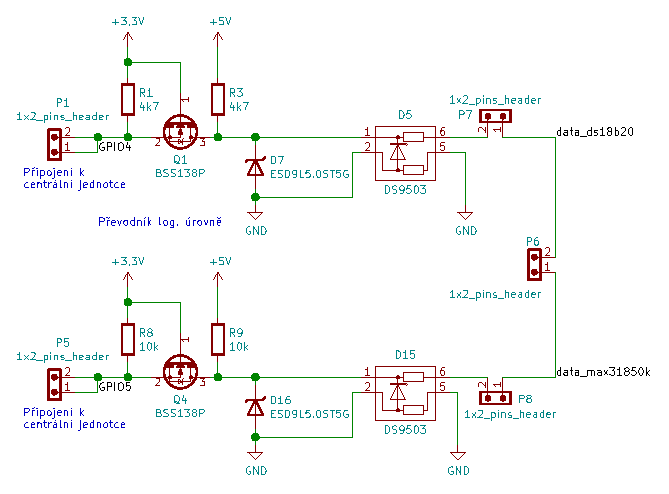
\includegraphics[width=0.9\textwidth]{images/svg/kicad/ochrany-1-wire.eps}
    \caption[ESD ochrany pro 1-Wire sběrnici s~převodníkem log. úrovní.]{ESD ochrany pro 1-Wire sběrnici s převodním log. úrovní. Kolíková lišta P1, P5 je připojena na Raspberry Pi.}
    \label{fig:ochrany-1-wire}
\end{figure}


\subsubsection{Napájení 1-Wire sběrnice}
\label{sec:napajeni-1-wire-sbernice}
Pro ochranu napájení 1-Wire sběrnice (5 V) jsou veškeré koncové teplotní senzory napájené přes elektronickou pojistku od Texas Instrumenst s označením TPS2600 \cite{tps26600}, schéma zapojení na obrázku \ref{fig:ochrana-napajeni-1-wire}. Obvod zajišťuje ochranu pro vstupní napětí, hlídá maximální hodnotu vstupního napětí do nastavené meze 5,25 V (maximální hranice je 60 V), minimální vstupní napětí do nastavené meze 4,75 V (minimální hranice je -60 V). Vstupní omezení napětí je pomocí rezistorů R5, R10, R11 a~R12. Omezovací proud je nastaven na přibližně 73~mA (hodnotu lze změnit přes potenciometr R17), při jeho překročení dojde k~odpojení výstupu po dobu, dokud nedojde k~odstranění závady. Kondenzátor C2 nastavuje rychlost náběhu výstupního napětí. Pro indikaci chyb napájení je červená LED.

\begin{figure}[H]
    \centering
    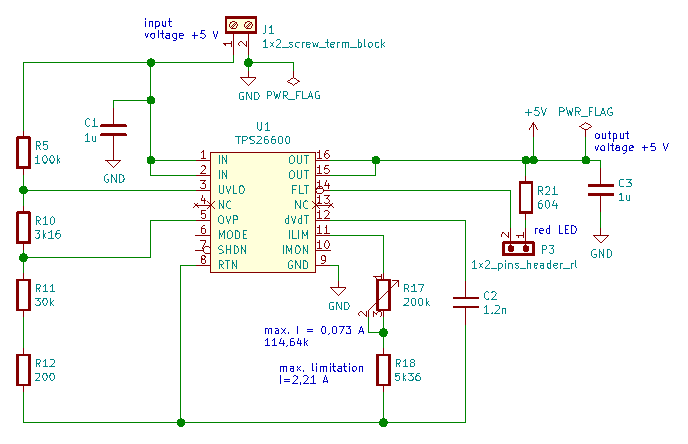
\includegraphics[width=\textwidth]{images/svg/kicad/ochrana-napajeni-1-wire.eps}
    \caption{Obvod TPS26600 pro ochranu napájení 1-Wire sběrnice.}
    \label{fig:ochrana-napajeni-1-wire}
\end{figure}

\subsubsection{Ochrana pro chodbové nástěnné termostaty}
Obdobně jako v části \ref{sec:datova-cast-1-wire-sbernice} (datová část 1-Wire sběrnice) je stejná ochrana pro snímání logické úrovně z~chodbových termostatů. Při sepnutí termostatu na daném patře je detekována log. 0 (požadavek na vytápění) v opačném případě je zde log. 1 (zastavení vytápění). Chodbové  termostaty jsou popsány v sekci \ref{sec:digitalni-chodbove-termostaty}.

\subsubsection{Ochrana napájení 3,3 V}
Přímo z Raspberry Pi je využito napětí 3,3 V pro převodník napětí, popsaný v~části \ref{sec:datova-cast-1-wire-sbernice} (datová část 1-Wire sběrnice). Zde je použita vratná pojistka polymerový \acrshort{ptc} (\textit{\acrlong{ptc}}) (RXEF005 \cite{rxef005}) se spínacím proudem 100 mA, pro omezení proudu v~případě poruchy, dále je zde transilová dioda (SM2T3V3A \cite{sm2t3v3a}) pro ochranu při přepětí (s~upínacím napětím max. 6,5~V (při 25 A, 10/1000~µs), průrazné napětí 3,6~V). Na obrázku \ref{fig:ochrana-napajeni-3_3-v} je zobrazena popsaná ochrana.

\begin{figure}[H]
    \centering
    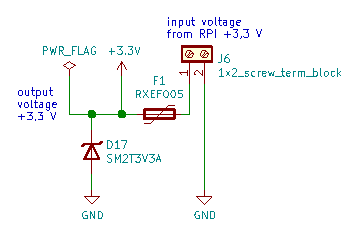
\includegraphics[width=0.6\textwidth]{images/svg/kicad/ochrana-napajeni-3_3-v.eps}
    \caption{Ochrana pro výstupní napětí 3,3 V z~Raspberry Pi.}
    \label{fig:ochrana-napajeni-3_3-v}
\end{figure}


\subsubsection{Realizovaná DPS ochran pro centrální jednotku Raspberry Pi}
Na obrázku \ref{fig:dps-pro-ochranu-vstupu-vystupu-pro-raspberry-pi} je realizovaná DPS vstupů/výstupů pro centrální jednotku Raspberry Pi. Ze samotné DPS je sběrnice vyvedena pomocí konektorů RJ45, čtyři konektory pro teplotní senzory DS18B20 a čtyři pro termočlánky s MAX31850K. Celkové schéma zapojení je v příloze \ref{app:schemata-ostatni}.

\begin{figure}[H]
\centering
\begin{subfigure}{.5\textwidth}
    \centering
    \includegraphics[width=0.6\textwidth]{images/vstupy-vystupu-rpi/dps-rpi-1-wire-termostaty-ochrany-spodek.png}
    \caption{Spodní část.}
    \label{fig:dps-rpi-1-wire-termostaty-ochrany-spodek}
\end{subfigure}%
\begin{subfigure}{.5\textwidth}
    \centering
    \includegraphics[width=0.7\textwidth]{images/vstupy-vystupu-rpi/dps-rpi-1-wire-termostaty-ochrany-vrsek.png}
    \caption{Vrchní část.}
    \label{fig:dps-rpi-1-wire-termostaty-ochrany-vrsek}
\end{subfigure}
\caption{DPS pro 1-Wire sběrnici a chodbové termostaty připojené k centrální jednotce.}
\label{fig:dps-pro-ochranu-vstupu-vystupu-pro-raspberry-pi}
\end{figure}

\section{Signalizace stavů u krbů}
\begin{figure}[H]
   \centering
    \def\svgwidth{0.3\columnwidth}
    \input{images/svg/otopna-soustava/vyrez-krb-signalizace.pdf_tex}
    \caption[Výřez pro umístění signalizace stavů u krbu.]{Výřez z obrázku \ref{fig:otopna-soustava-a-elektronika-rez-domu} – umístění signalizace stavů u krbu.}
    \label{fig:vyrez-krb-signalizace}
\end{figure}

Na obrázku \ref{fig:vyrez-krb-signalizace} je výřez části z celkového nákresu (obrázek \ref{fig:otopna-soustava-a-elektronika-rez-domu}) pro signalizaci stavů u krbu. Navržená DPS se skládá z části elektronické pojistky TPS2600, zapojení je obdobné jako v \ref{sec:napajeni-1-wire-sbernice} (napájení 1-Wire sběrnice), navíc je na vstupu připojena transilová dioda (ESD9L5.0ST5G). Napěťové meze jsou nastaveny stejně, tedy minimální napětí je 4,75 V, maximální 5,25 V, proud je omezen na maximální hodnotu 100 mA. Dále je zde přivedena 1-Wire sběrnice přes konektor RJ45 s~obdobnými ochranami jako v \ref{sec:datova-cast-1-wire-sbernice} (datová část 1-Wire sběrnice) pro připojení MAX31850K přes svorkovnici. V neposlední řadě jsou zde vstupy pro ovládání třech LED pro signalizaci (obrázek \ref{fig:led-indikace}) naakumulovaného zásobníku otopné vody, modrá LED signalizuje stav horní části zásobníku, oranžová LED je pro střední část, červená je pro signalizaci spodní části. Vstupní část je chráněná přes DS9503 a transilovou diodou (ESD9L5.0ST5G). Sepnutí LED je přes tranzistor (BSS138P). Obdobně jsou řešeny oranžová a modrá LED. Celkové schéma zapojení je v~příloze \ref{app:schemata-ostatni}.

\begin{figure}[H]
    \centering
    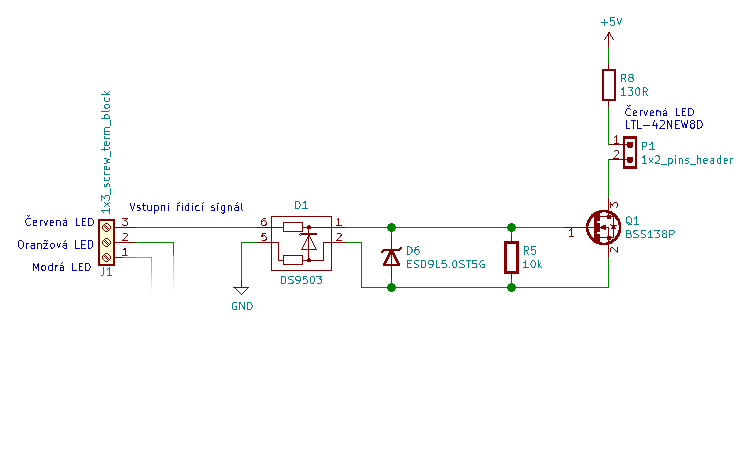
\includegraphics[width=\textwidth]{images/svg/kicad/led-indikace.eps}
    \caption{Zapojení pro ovládání signalizační červené LED.}
    \label{fig:led-indikace}
\end{figure}




\subsubsection{Měření teploty pomocí termočlánku a převodníku MAX31850K}
Teplotní senzory připojené na kouřovody krbů jsou realizované pomocí termočlánku z \ref{sec:teplotni-senzory-pro-krby}. Termočlánek je připojený k zakoupenému modulu (obrázek~\ref{fig:modul-max31850k-1-wire-prevodnik-termoclanku}), hodnota napětí z termočlánku je převedena do digitální podoby včetně teplotní kompenzace studeného konce a~tato hodnota je poslána po 1-Wire sběrnici. Je možné připojit termočlánek typu K. Převodník umožňuje měřit teplotu s~převodem pomocí AD převodníku až na 14 bitů. Rozlišení teploty činí 0,25~°C. Při teplotách -200 °C až 700 °C činí přesnost měřené teploty ±2~°C. Obvod disponuje detekcí zkratu (na GND nebo napájení) na vstupu pro termočlánek. Dále je zde detekce odpojeného termočlánku. Schéma zapojení modulu je v příloze \ref{app:schemata-ostatni}, upraveno z \cite{prevodnik-max31850k}.

%\begin{figure}[H]
%    \centering
%    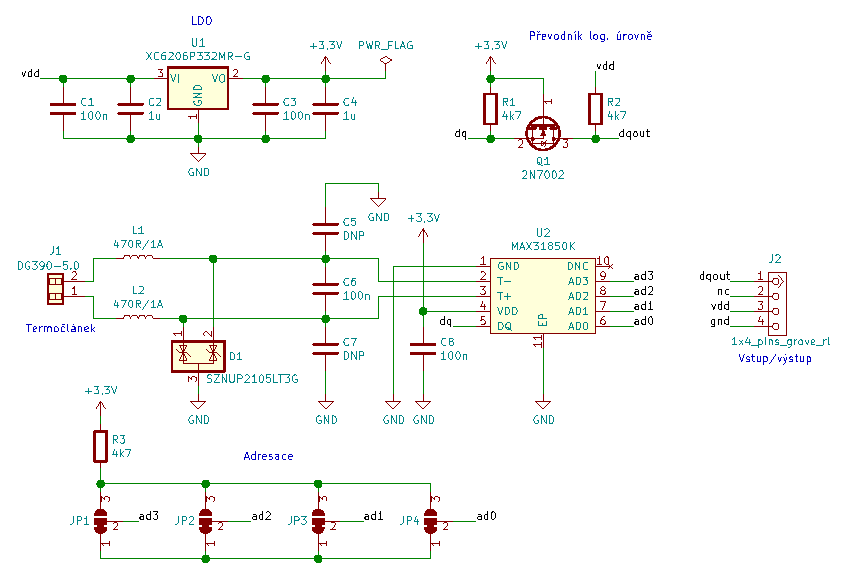
\includegraphics[width=\textwidth]{images/svg/kicad/zapojeni-max31850k-1-wire-prevodnik-termoclanku.eps}
%    \caption[Zapojení MAX31850K v modulu.]{Zapojení MAX31850K v modulu. Upraveno z \cite{prevodnik-max31850k}.}
%    \label{fig:zapojeni-max31850k-1-wire-prevodnik-termoclanku}
%\end{figure}

\begin{figure}[H]
    \centering
    \includegraphics[width=0.4\textwidth]{images/krb/modul-max31850k-1-wire-prevodnik-termoclanku.png}
    \caption[Modul s obvodem MAX31850K.]{Modul s obvodem MAX31850K \cite{prevodnik-max31850k}.}
    \label{fig:modul-max31850k-1-wire-prevodnik-termoclanku}
\end{figure}

\subsubsection{LCD displej}
Pro zobrazování teplot ze střední a spodní části zásobníku otopné vody byl zvolen 16 znakový a 2 řádkový LCD displej s modrým podsvícením a~bílými písmeny (obrázek \ref{fig:lcd-displej}). Pro obsluhu displeje slouží řadič HD44780. K~řadiči je připojen I$^2$C expandér PCF8574 s osmi výstupy, které jsou připojeny na datovou sběrnici pro ovládání respektive zobrazování znaků na displeji. Displej je zapojen za modulem popsaným v části \ref{sec:i2c-sbernice} (I$^2$C sběrnice). Každý displej, respektive expandér PCF8574 umožňuje nastavit pomocí propojek A0, A1, A2 unikátní adresu zařízení na sběrnici.

\begin{figure}[H]
\centering
\begin{subfigure}{.5\textwidth}
  \centering
  \includegraphics[width=0.91\linewidth]{images/krb/predni-cast-lcd-displeje.png}
  \caption{Přední část displeje.}
  \label{fig:predni-cast-lcd-displeje}
\end{subfigure}%
\begin{subfigure}{.5\textwidth}
  \centering
  \includegraphics[width=0.9\linewidth]{images/krb/zadni-cast-lcd-displeje-s-expanderem-pcf8574.png}
  \caption{Zadní část displeje s I$^2$C expandérem PCF8574.}
  \label{fig:zadni-cast-lcd-displeje-s-expanderem-pcf857}
\end{subfigure}
\caption[LCD displej pro zobrazování teplot ze zásobníku otopné vody.]{LCD displej pro zobrazování teplot ze zásobníku otopné vody \cite{lcd-displej}.}
\label{fig:lcd-displej}
\end{figure}

\subsubsection{Realizovaná DPS signalizace u krbů}
Výše popsané části jsou realizované na DPS (obrázek \ref{fig:dps-led-ochrany-u-krbu-spodek}, \ref{fig:dps-led-ochrany-u-krbu-vrsek}, \ref{fig:dps-led-ochrany-u-krbu-kabely}). Deska byla vlastnoručně navržena, vyrobena a osazena. Je aplikován ochranný lak. Celkové schéma zapojení je v příloze \ref{app:schemata-ostatni}.

\begin{figure}[H]
    \centering
    \includegraphics[width=0.8\textwidth]{images/krb/dps-led-ochrany-u-krbu-spodek.png}
    \caption{Spodní část DPS pro signalizaci u krbu.}
    \label{fig:dps-led-ochrany-u-krbu-spodek}
\end{figure}

\begin{figure}[H]
    \centering
    \includegraphics[width=0.8\textwidth]{images/krb/dps-led-ochrany-u-krbu-vrsek.png}
    \caption{Horní část DPS pro signalizaci u krbu.}
    \label{fig:dps-led-ochrany-u-krbu-vrsek}
\end{figure}

\begin{figure}[H]
    \centering
    \includegraphics[width=0.8\textwidth]{images/krb/dps-led-ochrany-u-krbu-kabely.png}
    \caption{DPS včetně signalizačních LED.}
    \label{fig:dps-led-ochrany-u-krbu-kabely}
\end{figure}

\subsubsection{Instalační krabice}
Všechna elektronika je umístěna do ochranné instalační krabice (obrázek \ref{fig:instalacni-krabice-vnitrek-krb}). Do krabice vstupují dva vodiče pro napětí 5 V a zem, tři kabely pro ovládání signalizačních LED, UTP kabel se sběrnicí 1-Wire pro teplotní senzor (termočlánek) a I$^2$C sběrnicí. Na obrázku \ref{fig:zadni-cast-krytu-vika-instalacni-krabice-krb} je zobrazena zadní část víka instalační krabice s uchycením signalizačních LED a LCD displeje. Na obrázku \ref{fig:predni-cast-krytu-vika-instalacni-krabice-krb} je přední část víka instalační krabice. Takto zkompletovaná instalační krabice je umístěna u krbu ve sklepě, v přízemí a v patře.

%\begin{figure}[H]
%    \centering
%    \includegraphics[width=0.6\textwidth]{images/krb/instalacni-krabice-vnitrek-krb.png}
%    \caption{Instalační krabice s jednotlivými moduly.}
%    \label{fig:instalacni-krabice-vnitrek-krb}
%\end{figure}

%\begin{figure}[H]
%    \centering
%    \includegraphics[width=0.6\textwidth]{images/krb/zadni-cast-krytu-vika-instalacni-krabice-krb.png}
%    \caption{Zadní část instalační krabice.}
%    \label{fig:zadni-cast-krytu-vika-instalacni-krabice-krb}
%\end{figure}



\begin{figure}[H]
\centering
\begin{subfigure}{.5\textwidth}
  \centering
  \includegraphics[width=0.835\textwidth]{images/krb/instalacni-krabice-vnitrek-krb.png}
  \caption{Instalační krabice s jednotlivými moduly.}
  \label{fig:instalacni-krabice-vnitrek-krb}
\end{subfigure}%
\begin{subfigure}{.5\textwidth}
  \centering
  \includegraphics[width=\textwidth]{images/krb/zadni-cast-krytu-vika-instalacni-krabice-krb.png}
  \caption{Zadní část instalační krabice.}
  \label{fig:zadni-cast-krytu-vika-instalacni-krabice-krb}
\end{subfigure}
\caption{Instalační krabice pro signalizaci stavů.}
\label{fig:instalacni-krabice}
\end{figure}



\begin{figure}[H]
    \centering
    \includegraphics[width=0.55\textwidth]{images/krb/predni-cast-krytu-vika-instalacni-krabice-krb.png}
    \caption[Víko instalační krabice.]{Víko instalační krabice. Osazený LCD displej, signalizačních LED (zleva modrá, oranžová a červená) a LED pro aktivování elektronické pojistky (červená LED vlevo od displeje).}
    \label{fig:predni-cast-krytu-vika-instalacni-krabice-krb}
\end{figure}




\section{Zónový regulátor}
Zónový regulátor se skládá s modulu PCA9615 (viz část \label{ses:i2c-sbernice} (I$^2$C)) pro realizaci I$^2$C sběrnice pomocí diferenciálních párů. Na modul je následně napojen zakoupený modul s obvodem PCA9685 od firmy NXP Semiconductors. Výstupy z modulu jsou napojeny na DPS, která zapíná/vypíná (respektive PWM regulace) jednotlivé termoelektrické pohony (celkově 12 pohonů, každý je řízen samostatně), čímž dochází k regulaci otopné vody do otopných okruhů. Zonové regulátory jsou umístěny u rozdělovače otopných okruhů v přízemí a~patře domu, celkově se jedná o dvě vyrobená zařízení.

\subsubsection{PCA9685}
Modul s obvodem PCA9685 umožňuje pomocí I$^2$C sběrnice ovládat 16 výstupů se stejnou individuální hodnotou PWM (se střídou 0 \% až 100 \%), frekvence je programovatelná od 24 Hz do 1\,526 Hz. Každý kanál navíc může dodat 10~mA jako source, případně 25 mA jako sink (což je 160 mA respektive 400~mA celkově).

\subsubsection{DPS pro ovládání termoelektrických pohonů}
Termoelektrické pohony jsou ovládány na základě hodnoty PWM z modulu PCA9685 (viz předchozí bod), každý výstupu ovládá jednotlivý pohon. Vzhledem k tomu, že termoelektrické pohony jsou na stejnosměrné napětí 24 V, je nutné využít napěťový převodník z 5 V na 24 V. K tomu slouží tranzistor MOSFET (DMN3023L-7). V závislosti na hodnotě PWM na jeho vstupu (gate) je otevírán/zavírán a dochází tak k regulaci napětí/proudu v~termoelektrickém pohonu, který je zapojen jako zátěž (přes drain). Paralelně k~tranzistoru se nachází přepínač, který slouží v případě poruchy k manuálnímu zapnutí/vypnutí pohonu. Přepínač má jmenovitý proud 0,5~A, což je dostatečné pro termoelektrický pohon, kterým při zapnutí teče maximální proud 250 mA (následně dochází ke snižování a saturaci proudu). Každý kanál obsahuje zelenou LED pro signalizaci, zda dochází k ovládání. Jak již bylo řečeno pohony jsou napájeny pomocí 24 V, jsou vytvořené dvě napájecí větve s obvodem TPC26600 (popsaný v části \ref{sec:napajeni-1-wire-sbernice}), rozdíl spočívá ve vstupním napájení, které činí 24 V. Jsou tedy rozdílné i~maximální a~minimální povolené meze, které činí max. 24,25 V a min. 10~V. Dále každá větev má nastavený maximální proud 1,5 A (každý pohon má maximální hodnotu proudu při zapnutí 250 mA pro celkově 6 pohonů na větev). Vzhledem k jednoduchosti obvodu TPS26600 a k jeho vlastnostem (především pro automatickou detekci odstranění závady, bez nutnosti restartu zařízení) bylo raději zvoleno zapojení se dvěma větvemi (maximální proud pro TPS26600 činí 2,21 A) než využití jiného integrovaného obvodu pro sloučení do jedné větve. Na obrázku \ref{fig:zonovy-regulator-mosfet-pwm-1-kanal} je zapojení jednoho kanálu pro ovládání termoelektrického pohonu.  Na obrázku \ref{fig:dps-zonovy-regulator-spodni-strana} spodní strana realizované DPS a na obrázku \ref{fig:zonovy-regulator-vrchni-strana} je vrchní strana, včetně osazeného modulu s obvodem PCA9615. Na obrázku \ref{fig:zonovy-regulator-spodni-strana} je spodní část panelu s DPS zonového regulátoru a na obrázku \ref{fig:zonovy-regulator-vrchni-strana} je čelní část panelu.  Celkové schéma zapojení je v příloze \ref{app:schemata-ostatni}. Umístění DPS v samotném rozdělovači pro přízemí je v příloze \ref{app:rozdelovac-podlahoveho-vytapeni}.


\begin{figure}[H]
    \centering
    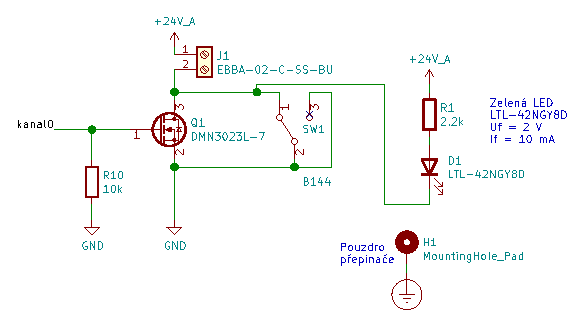
\includegraphics[width=\textwidth]{images/svg/kicad/zonovy-regulator-mosfet-pwm-1-kanal.eps}
    \caption{Zapojení jednoho kanálu pro ovládání termoelektrického pohonu.}
    \label{fig:zonovy-regulator-mosfet-pwm-1-kanal}
\end{figure}

\begin{figure}[H]
    \centering
    \includegraphics[width=0.99\textwidth]{images/zonovy-regulator/dps-zonovy-regulator-spodni-strana.png}
    \caption{DPS zonového regulátoru, spodní strana.}
    \label{fig:dps-zonovy-regulator-spodni-strana}
\end{figure}

\begin{figure}[H]
    \centering
    \includegraphics[width=0.99\textwidth]{images/zonovy-regulator/dps-zonovy-regulator-vrchni-strana.png}
    \caption{DPS zonového regulátoru, vrchní strana.}
    \label{fig:dps-zonovy-regulator-vrchni-strana}
\end{figure}


\begin{figure}[H]
    \centering
    \includegraphics[width=0.95\textwidth]{images/zonovy-regulator/zonovy-regulator-spodni-strana.png}
    \caption{Zadní část panelu zónového regulátoru.}
    \label{fig:zonovy-regulator-spodni-strana}
\end{figure}

\begin{figure}[H]
    \centering
    \includegraphics[width=0.95\textwidth]{images/zonovy-regulator/zonovy-regulator-vrchni-strana.png}
    \caption[Čelní část panelu zónového regulátoru.]{Čelní část panelu zónového regulátoru se signalizačními LED a~manuálním ovládáním pomocí spínačů.}
    \label{fig:zonovy-regulator-vrchni-strana}
\end{figure}



\subsubsection{Termoelektrické pohony Salus T30NC}  
Termoelektrický pohon Salus T30NC slouží k ovládání ventilů pro jednotlivé otopné okruhy. Je napájen stejnosměrným napětí 24 V při maximálním proudovém odběru při zapnutí 250 mA. Provozní příkon jsou 2 W. Rozměr závitu je M30\,×\,1,5. Maximální délka zdvihu pro dřík ventilu činí 4 mm. Síla pohonu je 100 N ($\pm$10 \%). Čas pro otevření je přibližně 2 minuty. Jedná se o~typ \acrshort{nc} (\textit{\acrlong{nc}}), při odpojení napájení je ventily zavřen. Pohon má funkci „First Open“ neboli je možné pomocí zarážky ventil instalovat jako otevřený bez nutnosti napájení (využít v případě, kdy není ještě instalovaná centrální jednotka). Pro každé patro je použito 12 těchto pohonů.

\begin{figure}[H]
    \centering
    \includegraphics[width=0.8\textwidth]{images/termoelektricky-pohon-salus-t30nc-24-v.png}
    \caption[Termoelektrický pohon Salus T30NC na stejnosměrné napětí 24 V.]{Termoelektrický pohon Salus T30NC na stejnosměrné napětí 24~V \cite{termoelektricky-pohon-t30nc}.}
    \label{fig:termoelektricky-pohon-salus-t30nc-24-v}
\end{figure}

\section{Digitální chodbové termostaty}
\label{digitalni-chodbove-termostaty}
Pro snímání teplot z jednotlivých pater na chodbách slouží digitální termostat s označením W3230. Termostat disponuje jedním spínací výstupem (v případě potřeby vytápění se výstup sepne, jinak je rozepnut). Je možné nastavit hysterezi, časové zpoždění, kalibraci teploty a rozsah maximálních teplot. Lze také aktivovat signalizaci, která se spustí po dosažení maximální přípustné teploty. Pro napájení je potřeba stejnosměrné napětí 12 V. Pro snímání teploty slouží NTC termistor. Rozsah teplot je -40 °C až 120 °C. Přesnost měření je $\pm$ 0,1 °C. Termostat lze nahradit za jakýkoliv jiný, který disponuje spínacím výstupem.


\begin{figure}[H]
    \centering
    \includegraphics[width=0.8\textwidth]{images/digitalni-termostat-w3230.png}
    \caption[Digitální termostat W3230.]{Digitální termostat W3230 \cite{digitalni-termostat-w3230}.}
    \label{fig:digitalni-termostat-w3230}
\end{figure}


\section{Spínací jednotka}
Pro spínání čerpadel a signalizačních LED slouží dva zakoupené relé moduly po čtyrech kanálech. Relé umožňují spínat výkony 250 VAC při max. 10~A a 30 V DC při max. 10~A. Jednotlivé kanály jsou oddělené galvanicky (dále je vyfrézovaná část DPS mezi výkonovou částí a spínací částí), též je možné využít různých zdrojů pro napájení spínací části a napájení relé. Zapojení jednoho kanálu je obrázku \ref{fig:rele-modul-jeden-kanal}. Celý relé modul je na obrázku \ref{fig:ctyr-kanalovy-rele-modul}.

\begin{figure}[H]
    \centering
    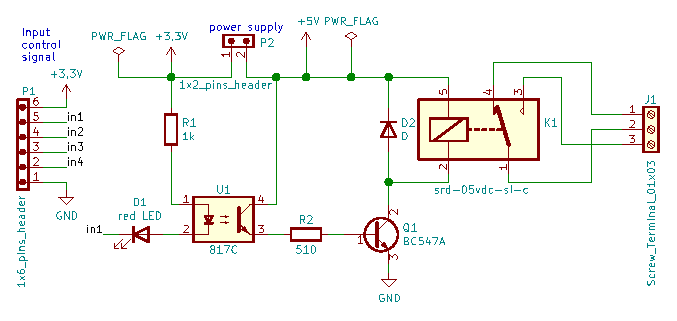
\includegraphics[width=\textwidth]{images/svg/kicad/rele-modul-jeden-kanal.eps}
    \caption{Zapojení jednoho kanálu relé modulu.}
    \label{fig:rele-modul-jeden-kanal}
\end{figure}


\begin{figure}[H]
    \centering
    \includegraphics[width=0.8\textwidth]{images/ctyr-kanalovy-rele-modul.png}
    \caption[Čtyř kanálový relé modul.]{Čtyř kanálový relé modul \cite{ctyr-kanalovy-rele-modul}.}
    \label{fig:ctyr-kanalovy-rele-modul}
\end{figure}

\section{Realizovaný rozvaděč s~elektronikou}

V realizovaném rozvaděči na obrázku \ref{fig:rozvadec-ve-sklepe-s-elektronikou} je umístěn 5 V zdroj pro napájení centrální jednotky, relé modulů, I$^2$C diferenciální sběrnice, napájení 1-Wire sběrnice a napájení elektroniky u krbů. Dále je zde 12 V zdroj pro napájení dvou lokálních chodbových termostatů. V  neposlední době jsou zde jističe pro jednotlivé zdroje a čerpadla včetně proudového chrániče.

\newpage

\begin{figure}[H]
    \centering
    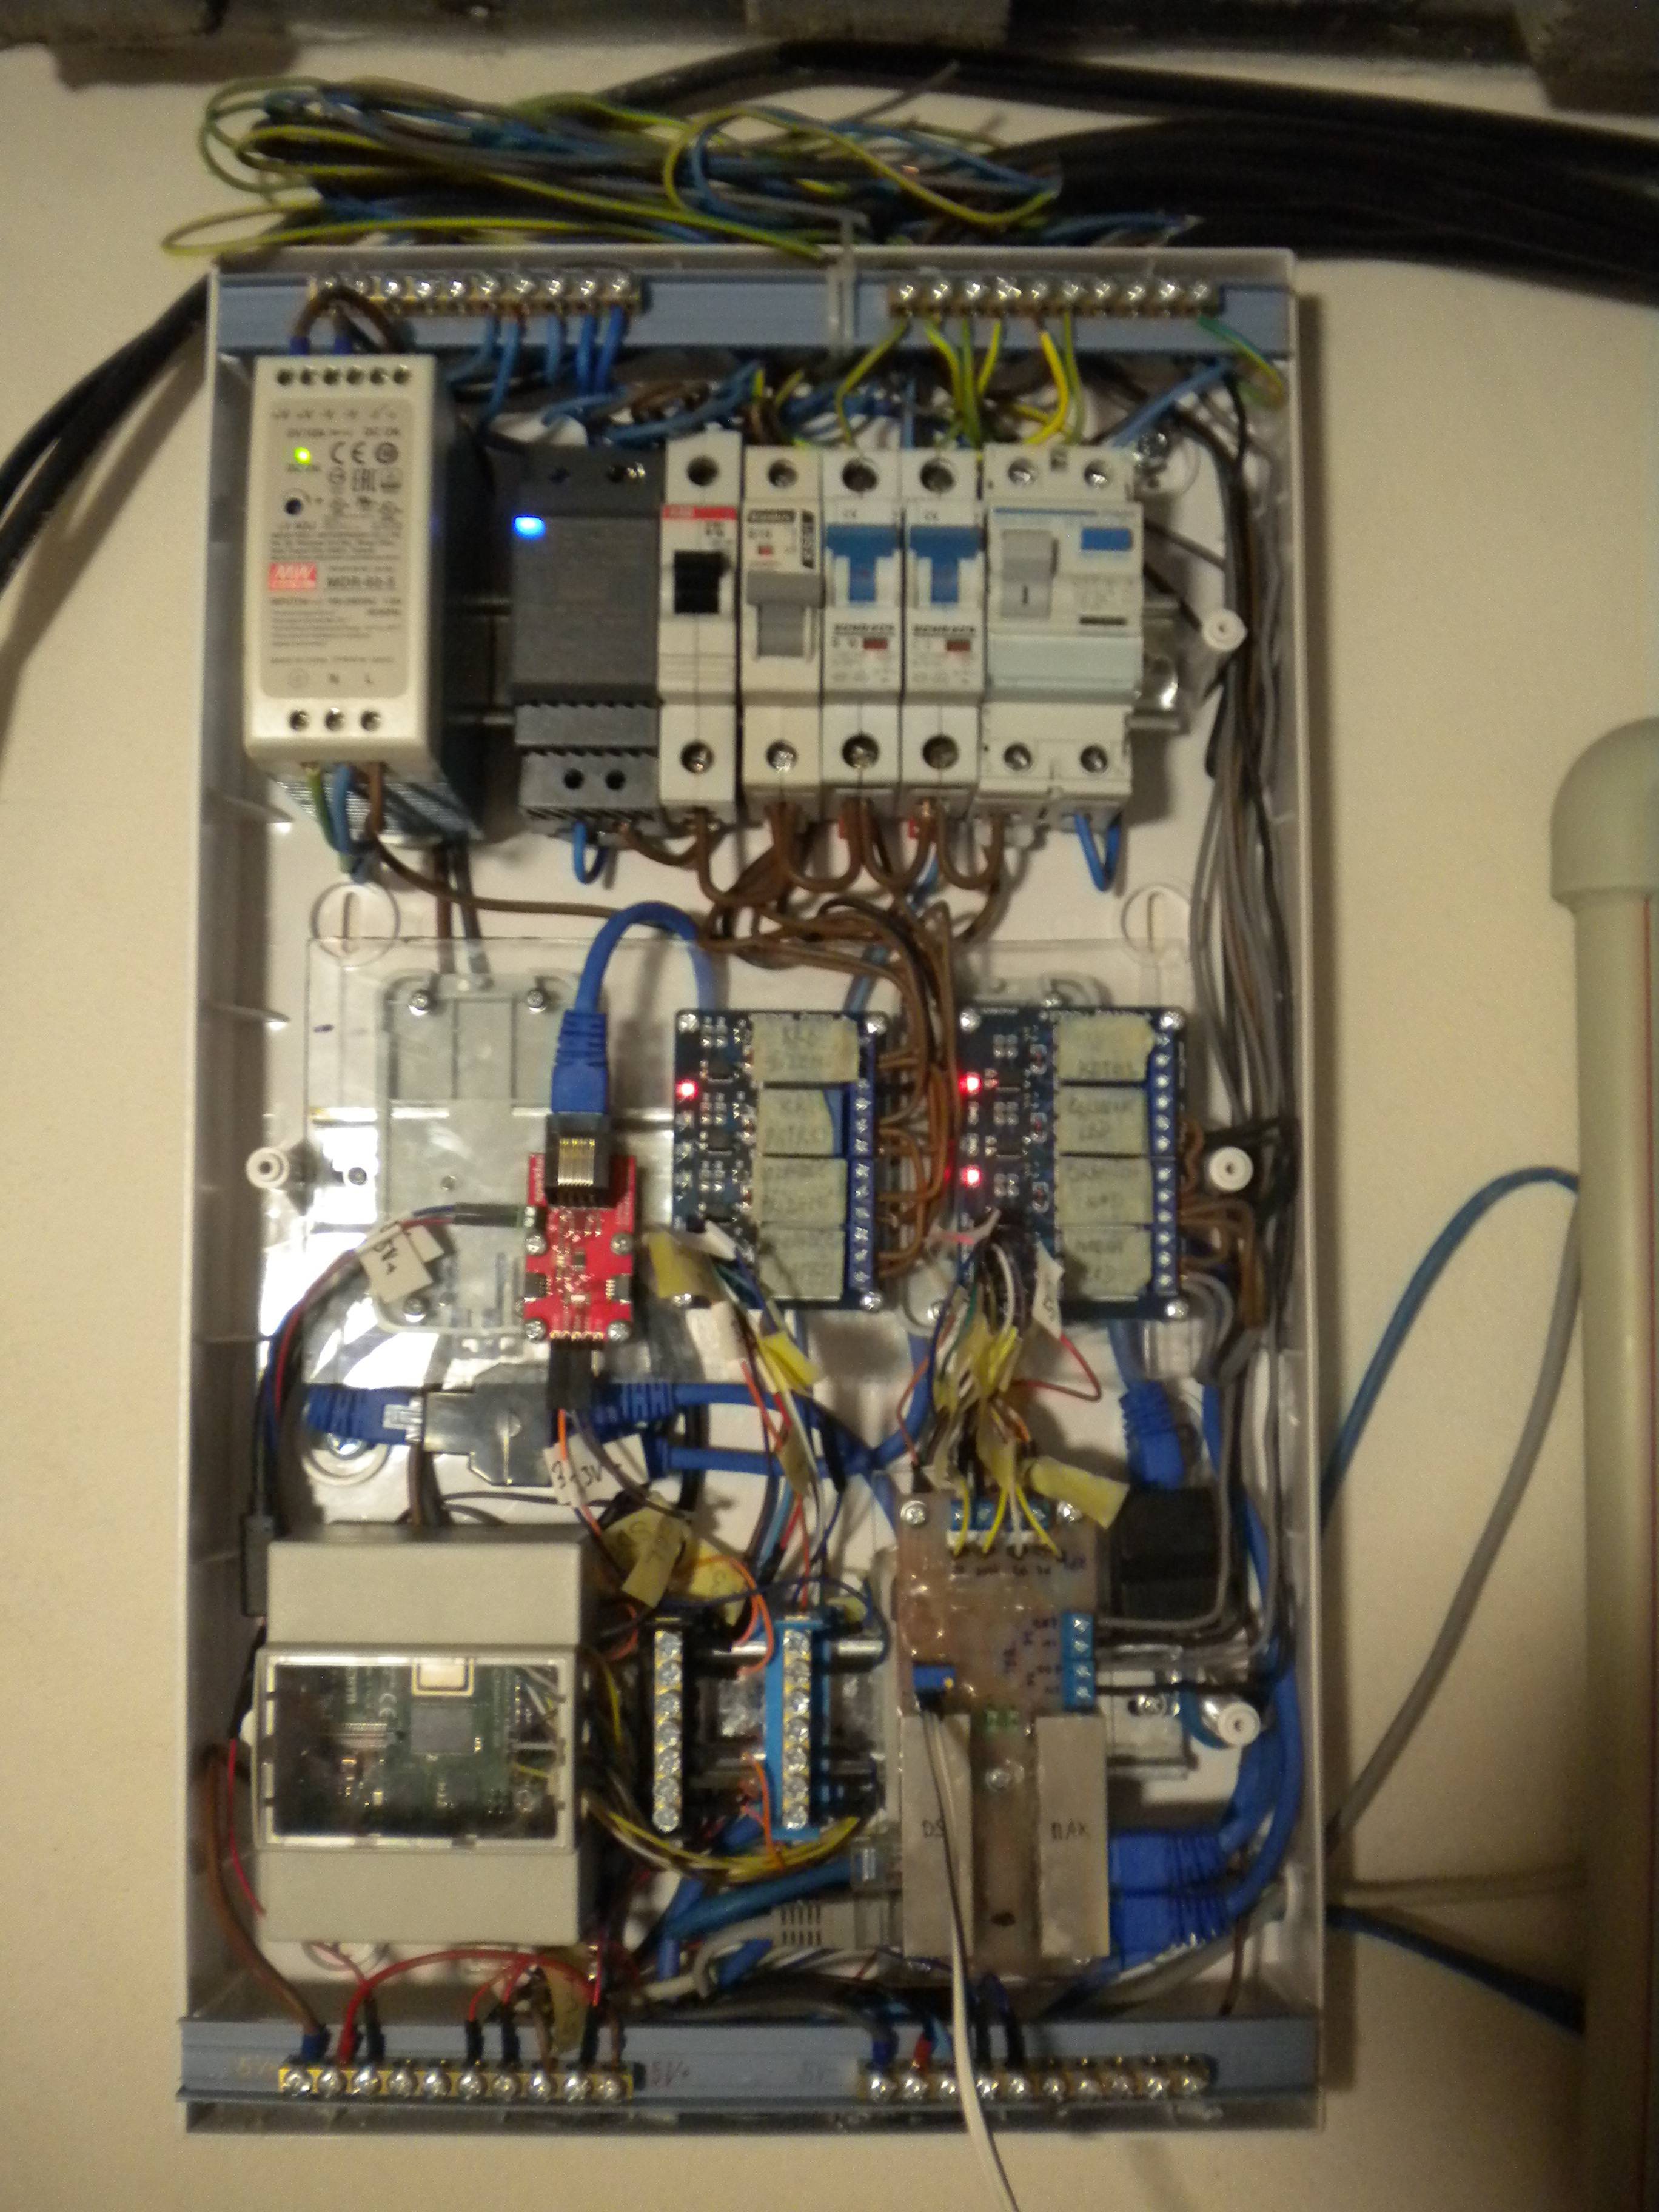
\includegraphics[width=0.99\textwidth]{images/rozvadec-ve-sklepe-s-elektronikou.png}
    \caption{Realizovaný rozvaděč s~elektronikou.}
    \label{fig:rozvadec-ve-sklepe-s-elektronikou}
\end{figure}


\section{Nástěnný snímač prostorové teploty}

Pro snímání prostorové teploty z místností slouží nástěnný snímač prostorové teploty. Tyto zařízení primárně slouží k měření teploty a její následné odesílání do centrální jednotky. Disponují tlačítky pro nastavení požadované teploty (změna teploty s~krokem 0,5 °C) pro danou místnost. Aktuálně naměřenou a požadovanou teplotu zobrazují uživateli přímo na displeji. V případě přenastavení v centrálním systému, dojde k propsání těchto změn přímo na jednotlivé snímací jednotky.  Nástěnný snímač prostorové teploty měří teplotu v místnosti každých 30~sekund. V případě síťového výpadku komunikace se zařízení automaticky snaží připojení obnovit, samotný výpad je signalizován i v centrální jednotce. Jednotky existují ve dvou variantách. První varianta komunikace s centrální jednotkou pomocí Ethernetu a je napájena pomocí aktivního \acrshort{poe} (\textit{\acrlong{poe}}). Druhá varianta komunikuje s centrální jednotkou pomocí bezdrátové sítě WiFi a je napájena pomocí síťového adaptéru. Obě varianty jsou popsány níže v sekci \ref{sec:ethernet-modul} a \ref{sec:wifi-modul}. Celkově je po domě umístěno 6 zařízení s Ethernetem a~4 zařízení s WiFi. DPS byly vlastnoručně navrženy, pro výrobu byla použita firma JLCPCB, součástky byly vlastnoručně osazeny.

\subsection{Varianta s Ethernetem}
\label{sec:ethernet-modul}

\begin{figure}[H]
   \centering
   \def\svgwidth{0.5\columnwidth}
   \input{images/svg/otopna-soustava/vyrez-nastenny-snimac-prostorove-teploty-ethernet.pdf_tex}
    \caption[Výřez pro umístění nástěnných snímačů prostorové teploty (verze Ethernet).]{Výřez z obrázku \ref{fig:otopna-soustava-a-elektronika-rez-domu} – umístění nástěnných snímačů prostorové teploty (verze Ethernet).}
    \label{fig:vyrez-nastenny-snimac-prostorove-teploty-ethernet}
\end{figure}

Na obrázku \ref{fig:vyrez-nastenny-snimac-prostorove-teploty-ethernet} je výřez části z celkového nákresu (obrázek \ref{fig:otopna-soustava-a-elektronika-rez-domu}) pro nástěnné snímače prostorové teploty (verze Ethernet). Na obrázku \ref{fig:blokove-schema-nastenny-snimac-teploty-ethernet} je blokové schéma nástěnného snímače prostorové teploty komunikující pomocí Ethernetu a je napájen pomocí aktivního POE. Snímač je napájen ze zařízení \acrshort{pse} (\textit{\acrlong{pse}}) (jedná se o POE switch MaxLink PSAT-10-8P-250 \cite{maxlink-psat-10-8p-250}), které řídí vykomunikování napájení a~výkonnostní třídy pro koncové zařízení (snímač (\acrshort{pd} (\textit{\acrlong{pd}}))). Jak zařízení PSE, tak PD podporují standart 802.3af \cite{norma-802.3af} respektive 802.3at \cite{norma-802.3at}. Zařízení PD jsou nastavená pro nejnižší definovanou výkonovou třídu 1 (max. výkon PSE pro jednotlivé PD zařízení je 4 W). Pro přenos napětí se využívají tzv. fantomové napětí, kdy v případě využití páru 1,2 a 3,6 se stejnosměrné napětí vyvede ze středu transformátoru. Další možností je využití volných párů 4,5 a 7,8 (zejména při rychlosti 10 nebo 100~Mbit/s (využity pro přenos dat 2 páry)). Vstupní napětí z PSE (44–57 V v~závislosti na délce kabelu UTP a~ztrátách) prochází přes diodový usměrňovač (nezávislost kladného pólu zdroje a země). Je zde řídící obvod TPS23753A \cite{tps23753a}, který zajišťuje komunikaci/rozhraní pro správné nastavení a povolení napětí z PSE, dále zajišťuje řízení převodu vstupního napětí na výstupní napětí 5~V (DC-DC měnič), je zapojen v~topologie Flyback (využívá tedy vázaný induktor). Zpětná vazba je řešena pomocí optické zpětné vazby s nastavitelnou Zenerovou diodou TLV431A \cite{tlv431a} v~zapojení komparátoru. Při návrh zdrojové části zařízení jsem vycházel z referenčního návrhu od výrobce Texas Instruments pro integrovaný obvod TPS23753A.

Zařízení v provozu je primárně  napájeno pomocí 5 V, v případě programování zařízení je možné použít programovací konektor s napájecím pinem pro 5 V. Pokud je k~dispozici POE, dojde zablokování napájení z programovacího konektoru (pomocí MOSFETu s~kanálem P). Napětí 5 V je následně vedeno do dvou \acrshort{ldo} (\textit{\acrlong{ldo}}) regulátorů. Jeden slouží pouze pro napájení ESP32 \cite{esp32-wrover-ie} modulu, druhý je pro napájení zbylých periferií (displej, tlačítka, teplotní senzor, obvod pro fyzickou vrstvu Ethernetu W5500 \cite{w5500}). Důvodem rozdělení je proudové rozdělení jednotlivých regulátorů a tedy i jejich ztrátové teplo. Vzhledem k parametrům udávané výrobcem modulu ESP32 je možné max. proudový odběr až 0,5~A (proto byl vybrán regulátor, který toto zatížení dlouhodobě zvládne při daném úbytku napětí i když se reálně nepředpokládá, že k tomuto zatížení dojde). Dále bylo zohledněno, pokud by došlo k ESD události (jedná se o~zařízení na které uživatelé sahají), tak je žádoucí, aby došlo maximálně k~restartu periferií a ne k restartu samotného ESP32 modulu. 

Pro programování modulu je zde konektor pro připojení externího modulu (viz část \ref{sec:prevodnik-usb-uart-cp2102n}), kde jsou piny pro TX/RX signál z UART a signály na automatický reset a boot modulu a piny pro napájení 5 V a země. Dále jsou zde přímo na DPS umístěná tlačítka pro boot a reset ESP32 modulu bez závislosti připojení programovacího modulu (lze tedy programovat i jinými moduly, které nemají automatický reset a boot). 

Samotné zařízení disponujeme ohranými transily na místech konektorů a~částí, které jsou přímo v kontaktu s uživatelem. Samotný obvod pro POE též disponuje proudovou a teplotní ochranou. LDO regulátory disponují detekcí nízkého vstupního napětí pro úspěšné spuštění, teplotní pojistkou a ochranou při zvýšení výstupního napětí vůči vstupnímu. 

Pro zobrazování aktuální a požadované teploty jsem zvolil barevný TFT displej velikosti 2.2" (240×320 pixelů) s řadičem ILI9341 \cite{lcd-ili9341}. Displej je připojen k~ESP32 modulu pomocí SPI sběrnice. Displej disponuje možností ovládání podsvícení pomocí PWM. Pro fyzickou vrstvu slouží obvod W5500, který implementuje ethernetový řadič s integrovaným TCP/IP. Obvod je s modulem ESP32 připojen pomocí SPI sběrnice. Pro snímání teploty slouží teplotní senzor DS18B20 (viz sekce \ref{sec:teplotni-senzory-pro-krby}). V neposlední řadě jsou zde tři tlačítka pro nastavení požadované teploty a~vyvolání nabídky menu.

Modul ESP32 disponuje rozhraním \acrshort{rmii} (\textit{\acrlong{rmii}}), který má složitější softwarovou implementaci a využívá větší počet pinů. Proto jsem zvolil integrovaný obvod W5500. Použití i využití následných knihoven bylo mnohem jednodušší. Vzhledem k malému vytížení komunikace je tento obvod dostačující. Pro komunikace mezi modulem ESP32 a displejem a obvodem W5500 jsou využity dvě nezávislé SPI sběrnice. 

V příloze \ref{app:nastenny-snimac-prostorove-teploty-ethernet} je schéma snímací jednotky. Na obrázku \ref{fig:dps-nastenny-snimac-prostorove-teploty-ethernet-vrchni-cast} je vrchní část realizované DPS pro snímací jednotku. Pro lepší galvanické oddělení jsou vyfrézované drážky. Dále na obrázku \ref{fig:dps-nastenny-snimac-prostorove-teploty-ethernet-vrchni-cast-displej} je DPS s osazeným displejem. Na obrázku \ref{fig:dps-nastenny-snimac-prostorove-teploty-ethernet-spodni-cast} je spodní část DPS. Kompletní zařízení včetně umístění do krabičky a popis samotné krabičky je v části \ref{sec:krabicka-pro-nastenny-snimac-prostorove-teploty}.



\begin{figure}[H]
    \centering
    \def\svgwidth{\columnwidth}
    \input{images/svg/blokove-schema-nastenny-snimac-teploty-ethernet.pdf_tex}
    \caption[]{Blokové schéma nástěnného snímače prostorové teploty (verze Ethernet).}
    \label{fig:blokove-schema-nastenny-snimac-teploty-ethernet}
\end{figure}


\begin{figure}[H]
\centering
\begin{subfigure}{.5\textwidth}
  \centering
  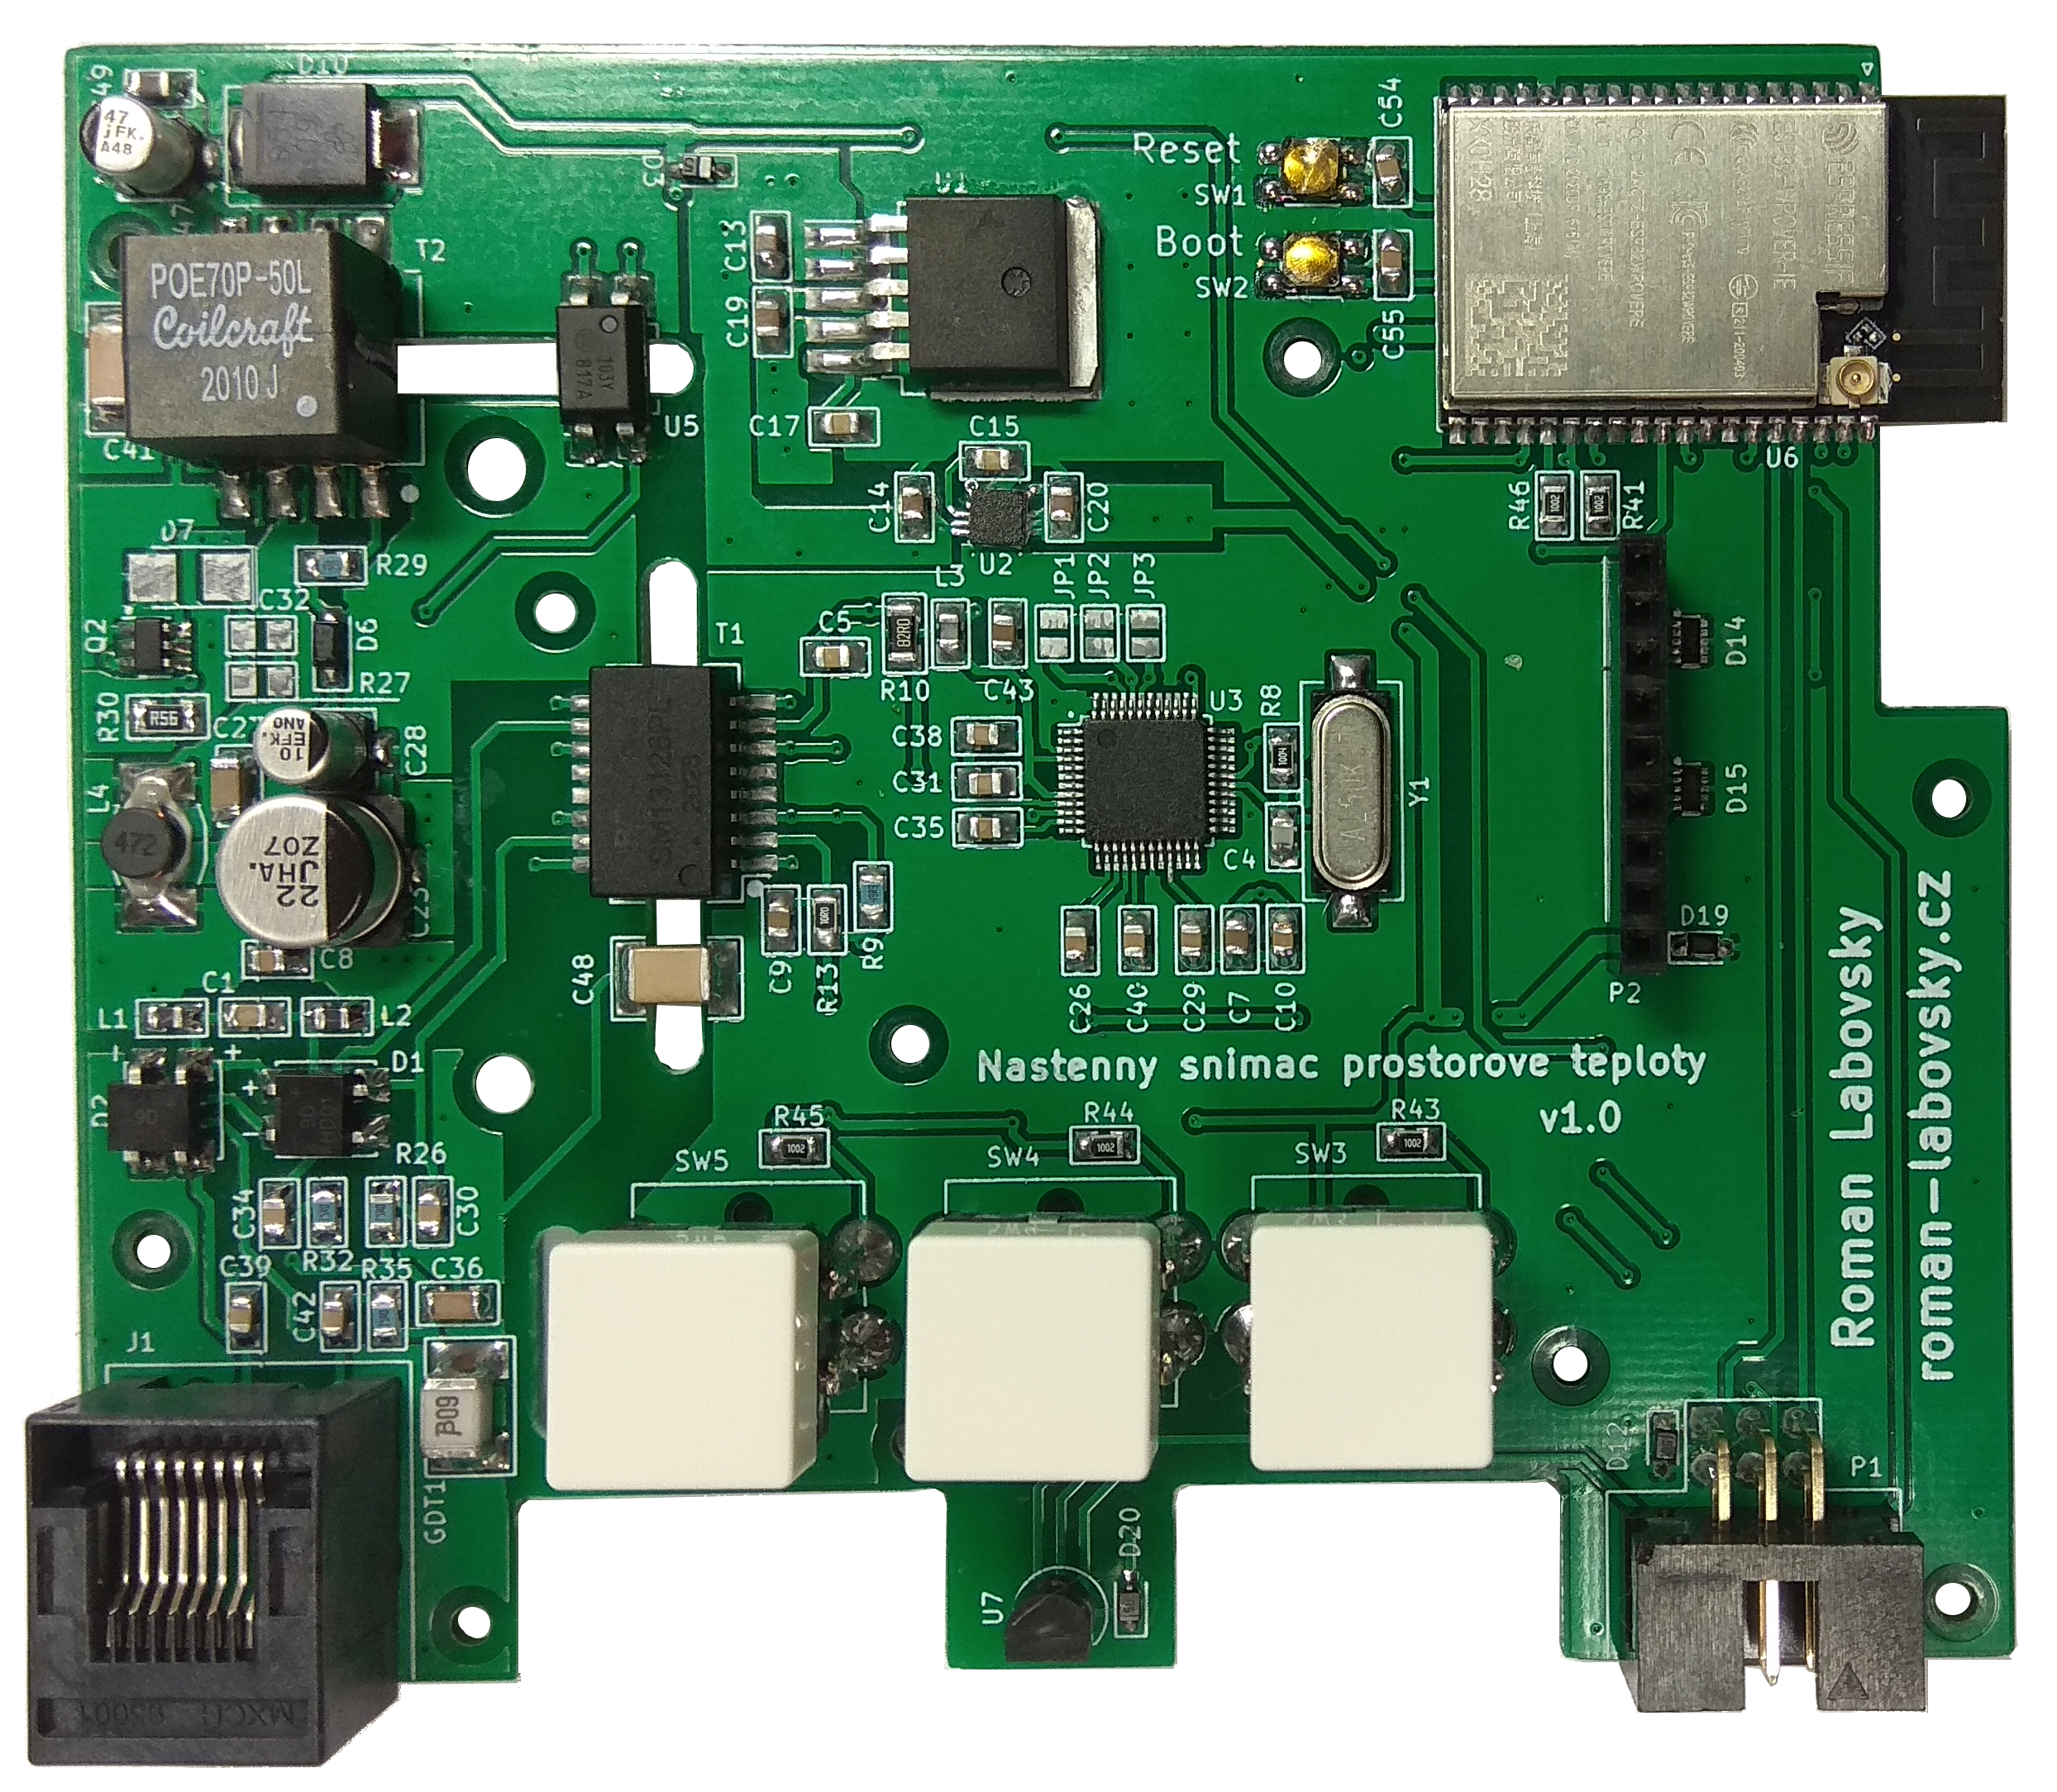
\includegraphics[width=\textwidth]{images/nastenny-snimac-prostorove-teploty-ethernet/dps-nastenny-snimac-prostorove-teploty-ethernet-vrchni-cast.png}
  \caption{Vrchní strana.}
  \label{fig:dps-nastenny-snimac-prostorove-teploty-ethernet-vrchni-cast}
\end{subfigure}%
\begin{subfigure}{.5\textwidth}
  \centering
  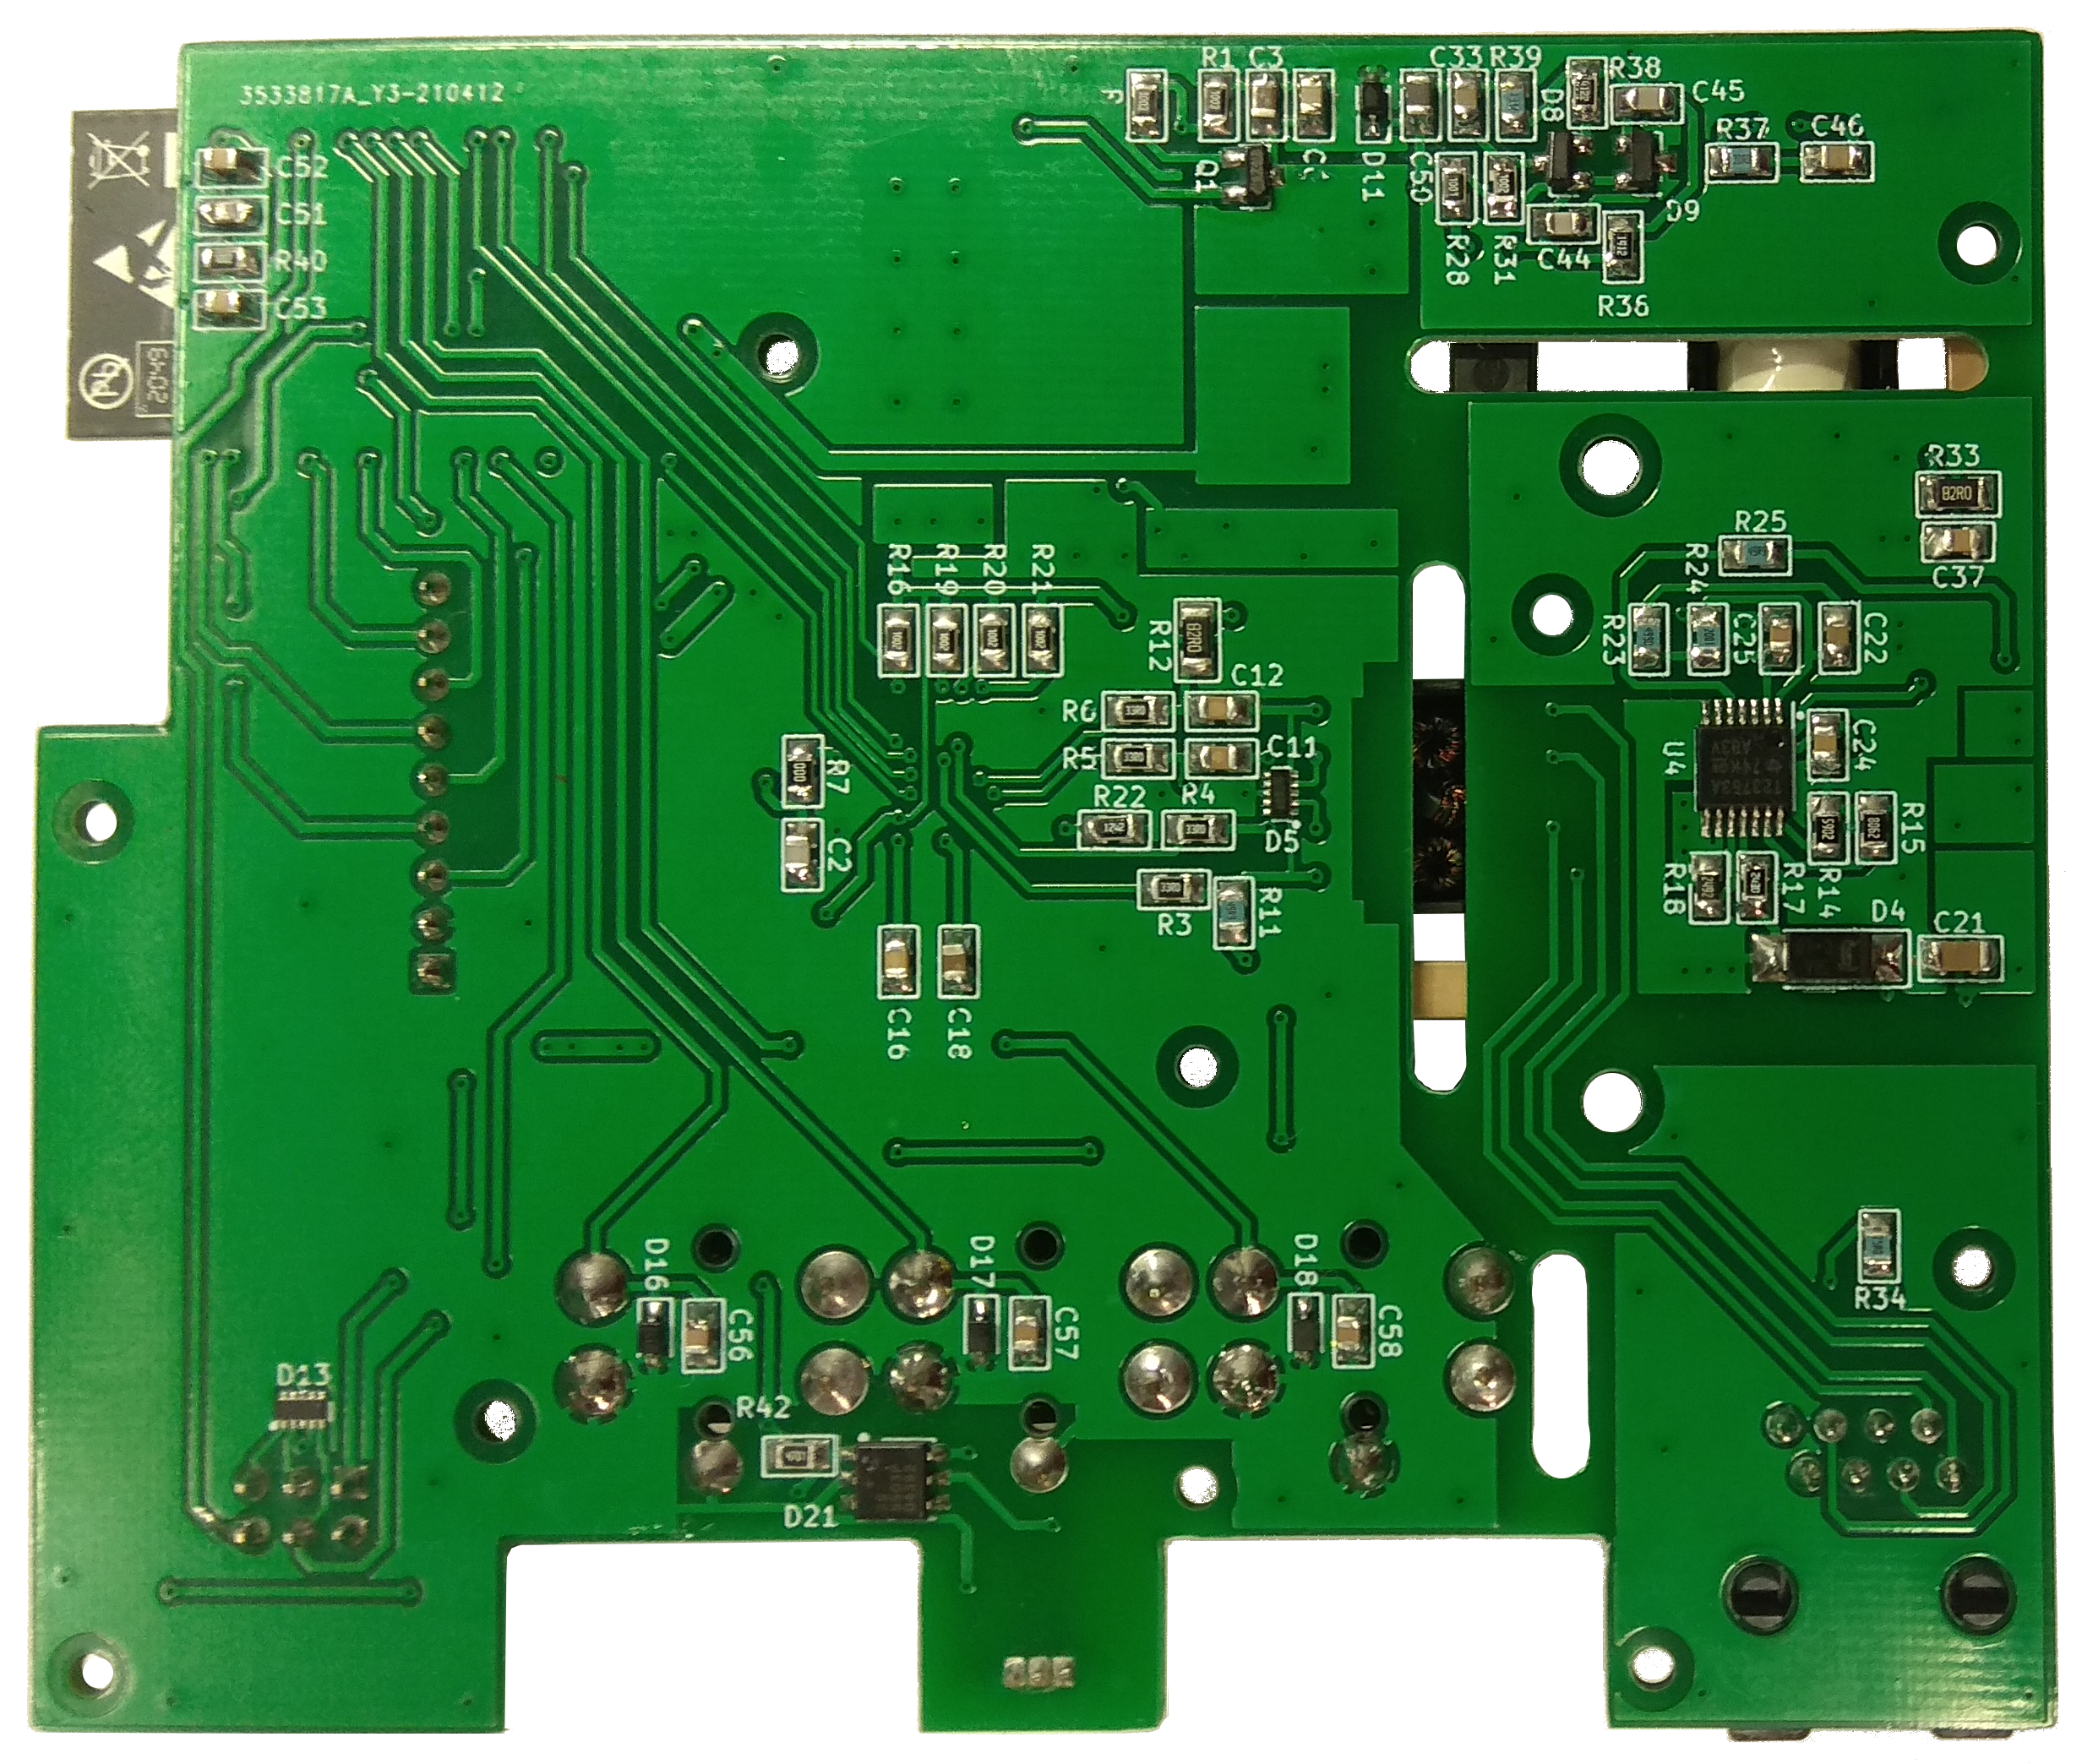
\includegraphics[width=\textwidth]{images/nastenny-snimac-prostorove-teploty-ethernet/dps-nastenny-snimac-prostorove-teploty-ethernet-spodni-cast.png}
  \caption{Spodní strana.}
  \label{fig:dps-nastenny-snimac-prostorove-teploty-ethernet-spodni-cast}
\end{subfigure}
\caption{DPS nástěnného snímače prostorové teploty (verze Ethernet).}
\label{fig:dps-nastenny-snimac-prostorove-teploty-ethernet}
\end{figure}


\begin{figure}[H]
    \centering
    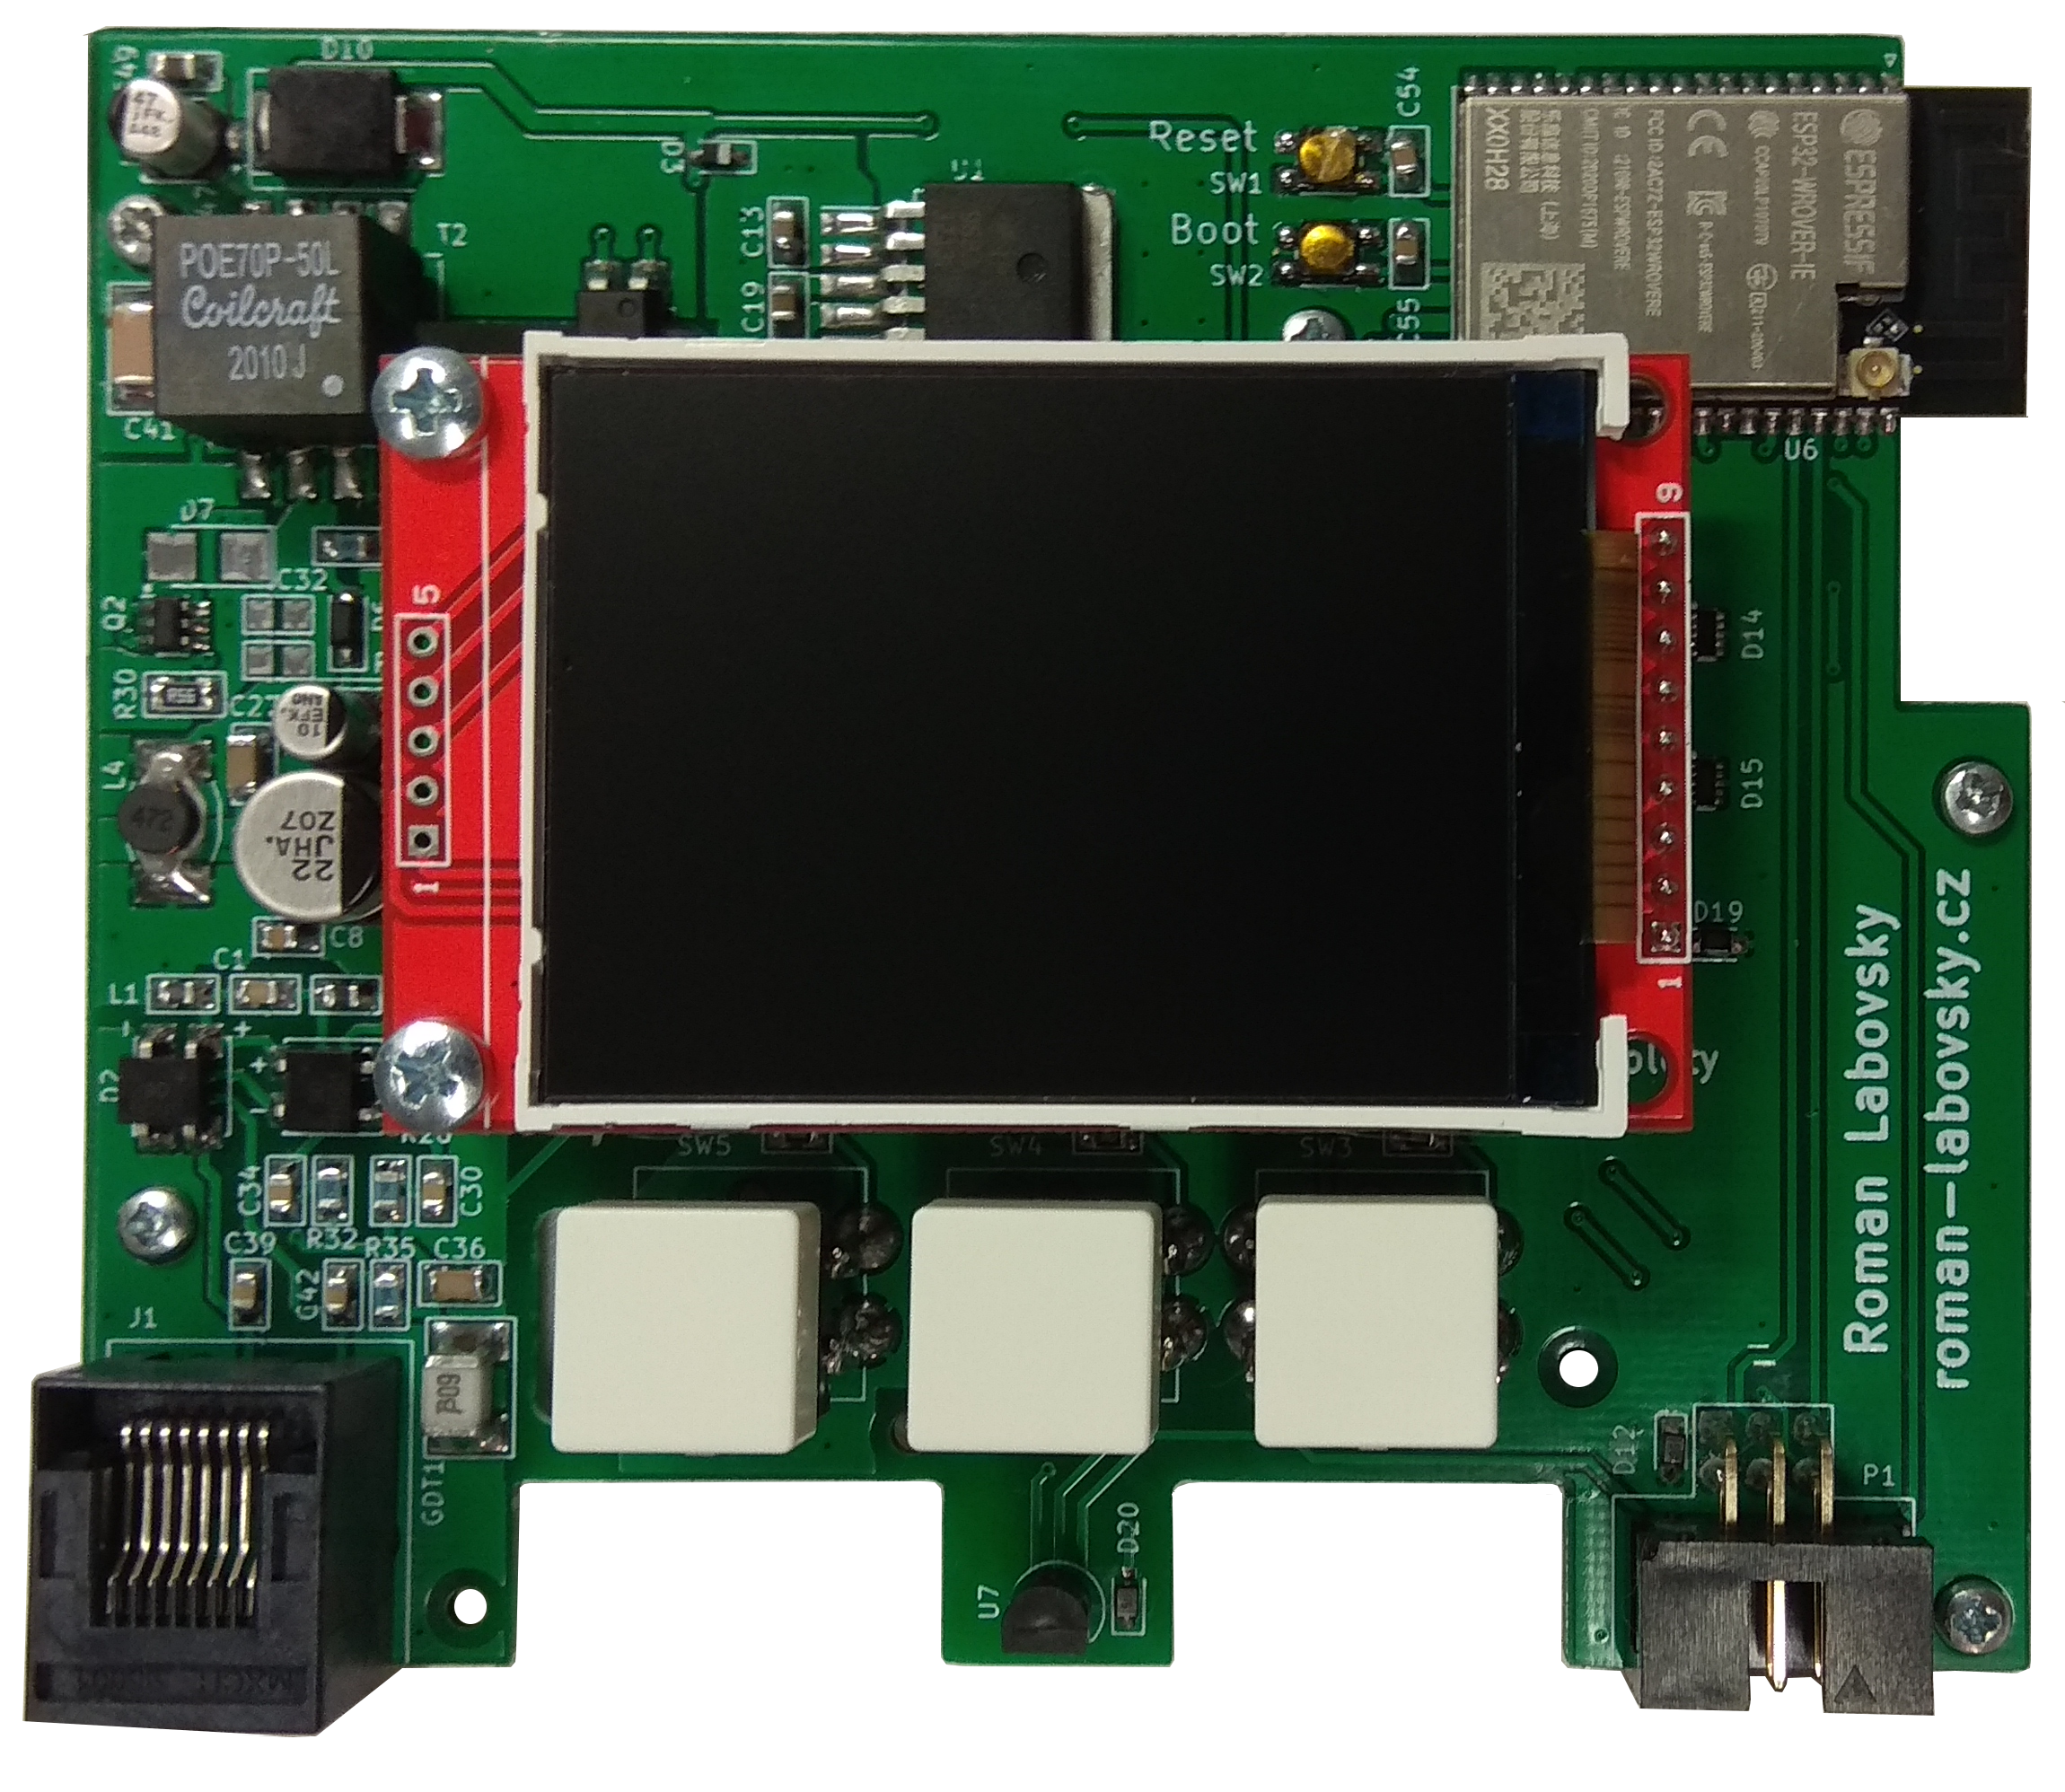
\includegraphics[width=0.88\textwidth]{images/nastenny-snimac-prostorove-teploty-ethernet/dps-nastenny-snimac-prostorove-teploty-ethernet-vrchni-cast-displej.png}
    \caption{DPS nástěnného snímače prostorové teploty (verze Ethernet) s~displejem, vrchní strana.}
    \label{fig:dps-nastenny-snimac-prostorove-teploty-ethernet-vrchni-cast-displej}
\end{figure}



\subsection{Varianta s WiFi}
\label{sec:wifi-modul}


\begin{figure}[H]
   \centering
   \def\svgwidth{0.5\columnwidth}
   \input{images/svg/otopna-soustava/vyrez-nastenny-snimac-prostorove-teploty-wifi.pdf_tex}
    \caption[Výřez umístění nástěnných snímačů prostorové teploty (verze WiFi).]{Výřez z obrázku \ref{fig:otopna-soustava-a-elektronika-rez-domu} – umístění nástěnných snímačů prostorové teploty (verze WiFi).}
    \label{fig:vyrez-nastenny-snimac-prostorove-teploty-wifi}
\end{figure}

Na obrázku \ref{fig:vyrez-nastenny-snimac-prostorove-teploty-wifi} je výřez části z celkového nákresu (obrázek \ref{fig:otopna-soustava-a-elektronika-rez-domu}) systému znázorňující umístění nástěnných snímačů prostorové teploty (verze WiFi). Na obrázku \ref{fig:blokove-schema-nastenny-snimac-teploty-wifi} je blokové schéma nástěnného snímače prostorové teploty komunikující pomocí WiFi a je napájen pomocí síťového adaptéru (Mean Well GSM06E05-P1J \cite{gsm06e05-p1j}). Oproti verzi z \ref{sec:ethernet-modul} chybí celá část tykající se POE napájení a také obvod W5500 implementující ethernetovou komunikaci. Zbylé části jsou totožné jako v části \ref{sec:ethernet-modul}.

V příloze \ref{app:nastenny-snimac-prostorove-teploty-wifi} je schéma snímací jednotky. Na obrázku \ref{fig:dps-nastenny-snimac-prostorove-teploty-wifi-vrchni-cast} je vrchní část realizované DPS pro snímací jednotku. Dále na obrázku \ref{fig:dps-nastenny-snimac-prostorove-teploty-wifi-vrchni-cast-displej} je DPS s osazeným displejem. Na obrázku \ref{fig:dps-nastenny-snimac-prostorove-teploty-wifi-spodni-cast} je spodní část DPS. Kompletní zařízení včetně umístění do krabičky a popis samotné krabičky je v části \ref{sec:krabicka-pro-nastenny-snimac-prostorove-teploty}.

\begin{figure}[H]
    \centering
    \def\svgwidth{\columnwidth}
    \input{images/svg/blokove-schema-nastenny-snimac-teploty-wifi.pdf_tex}
    \caption[]{Blokové schéma nástěnného snímače prostorové teploty (verze WiFi).}
    \label{fig:blokove-schema-nastenny-snimac-teploty-wifi}
\end{figure}


\begin{figure}[H]
\centering
\begin{subfigure}{.5\textwidth}
  \centering
    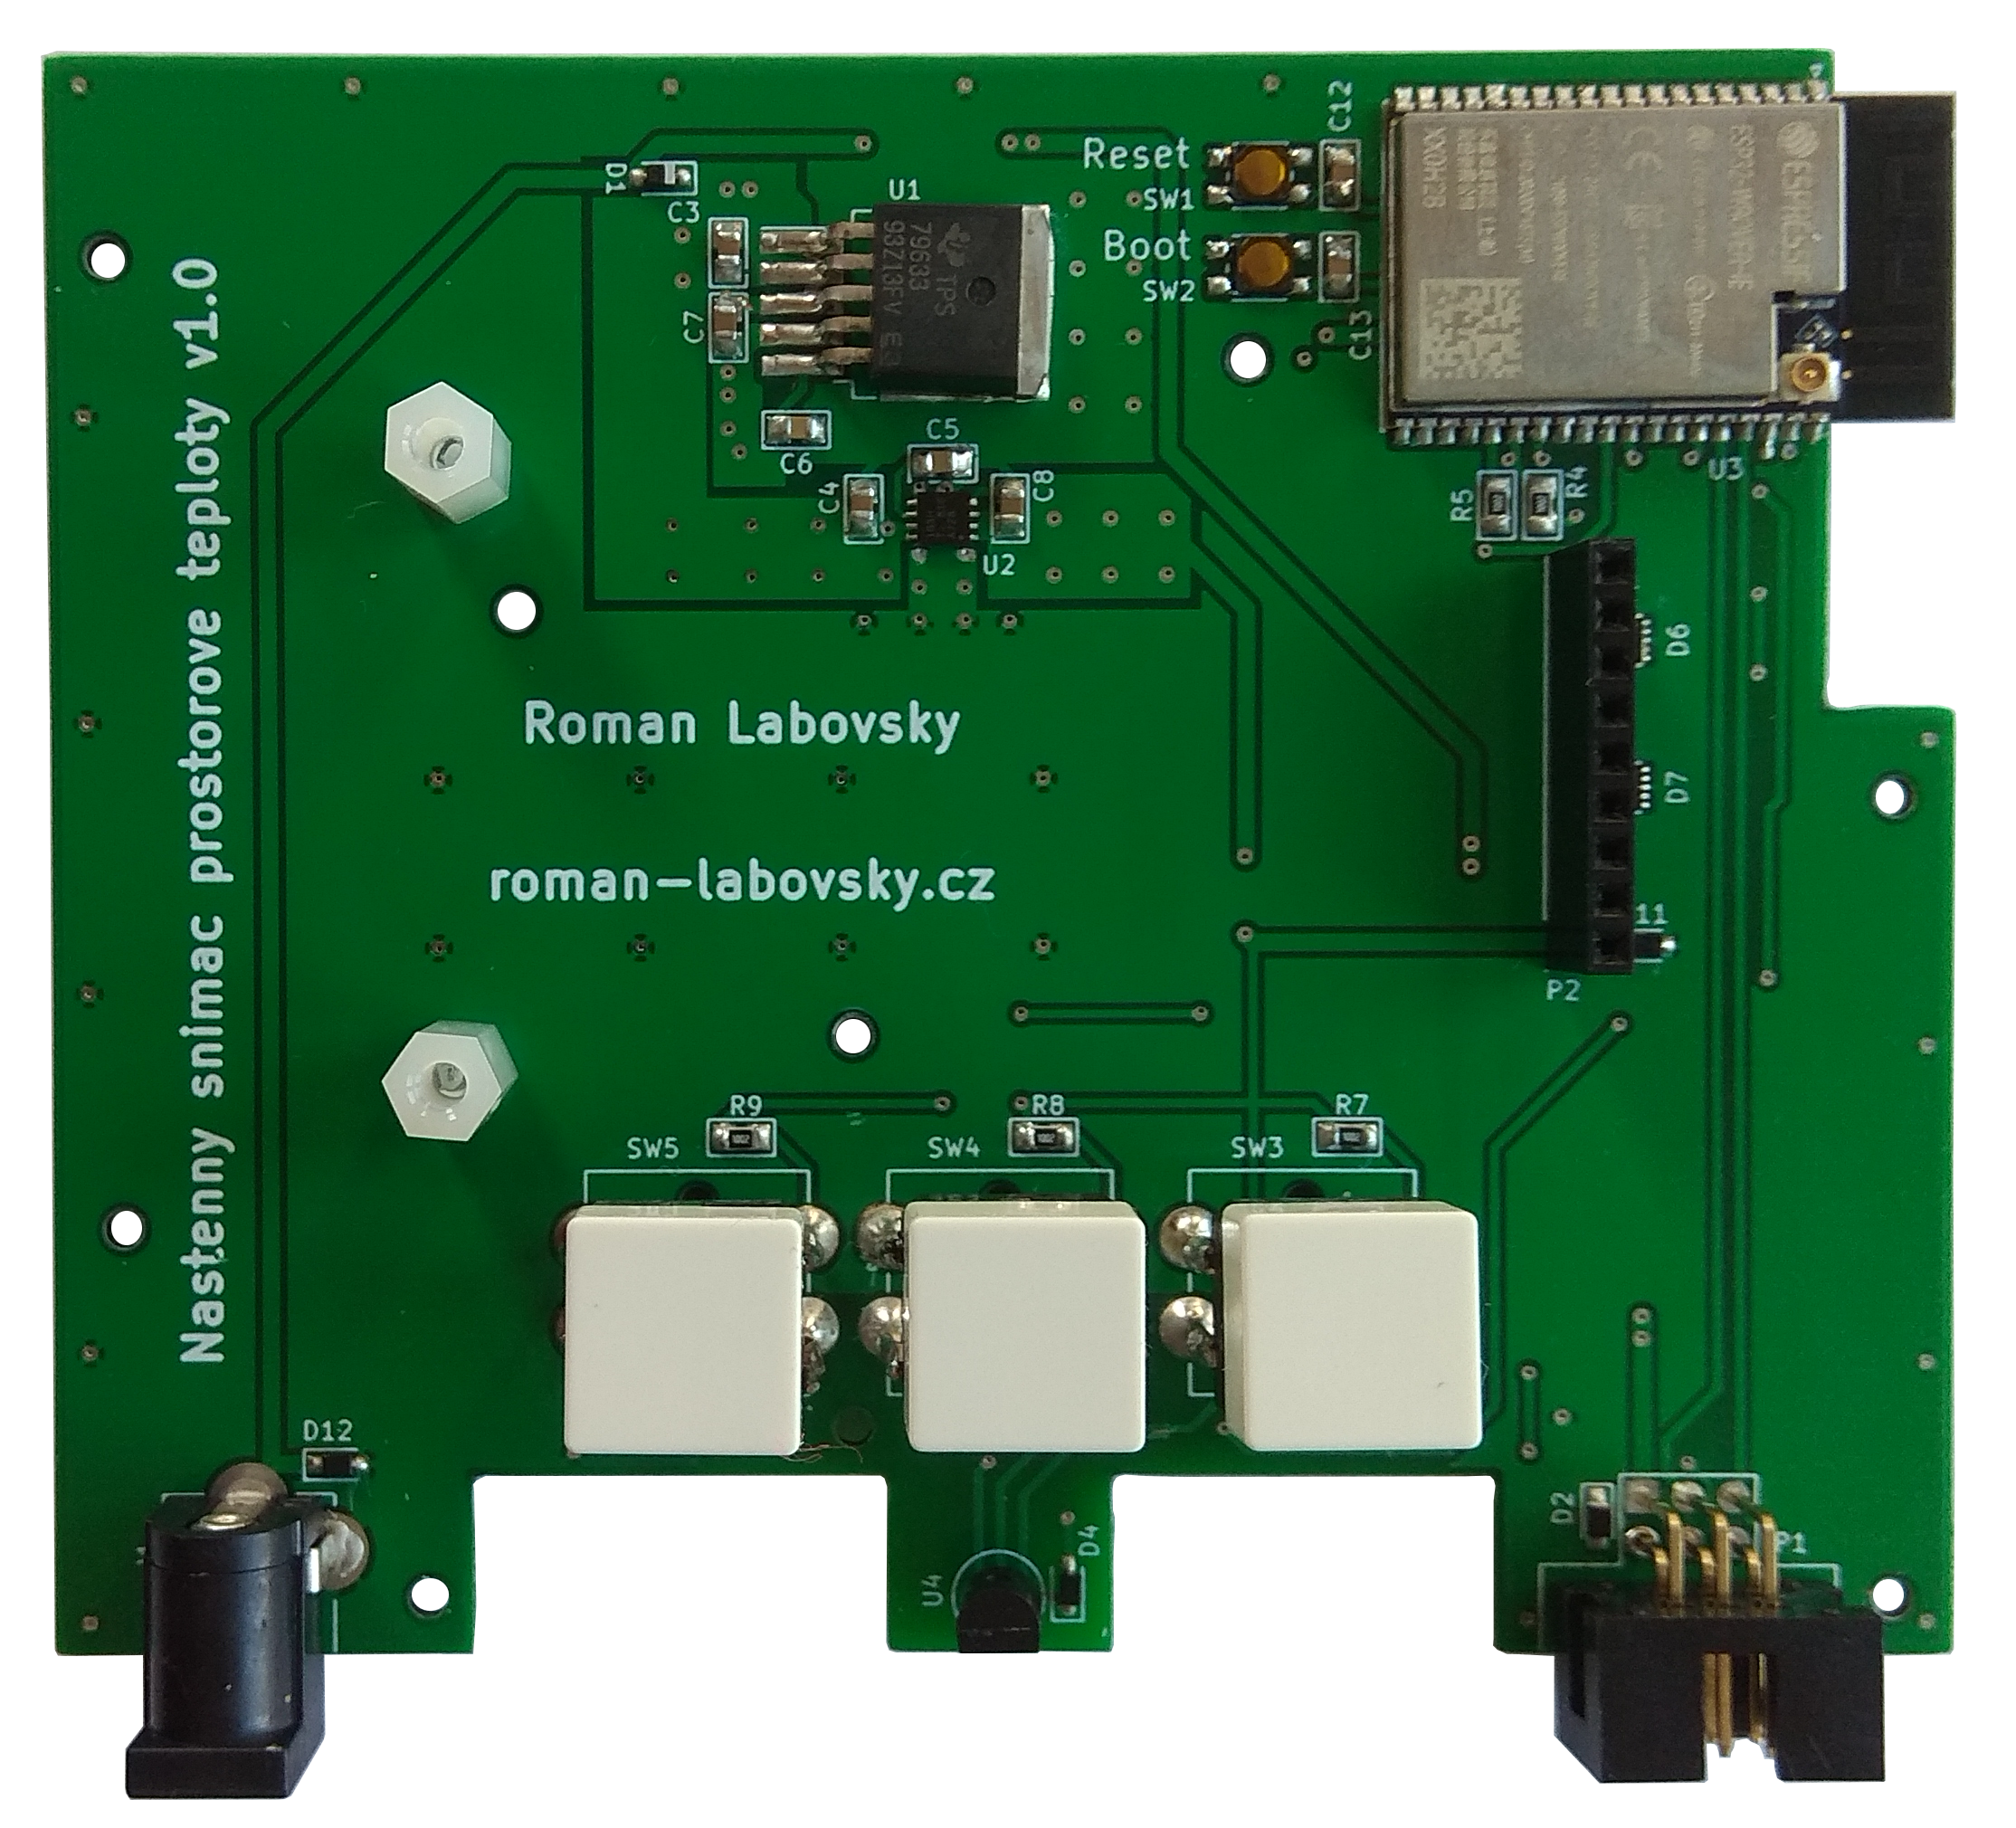
\includegraphics[width=\textwidth]{images/nastenny-snimac-prostorove-teploty-wifi/dps-nastenny-snimac-prostorove-teploty-wifi-vrchni-cast.png}
    \caption{Vrchní strana.}
    \label{fig:dps-nastenny-snimac-prostorove-teploty-wifi-vrchni-cast}
\end{subfigure}%
\begin{subfigure}{.5\textwidth}
  \centering
    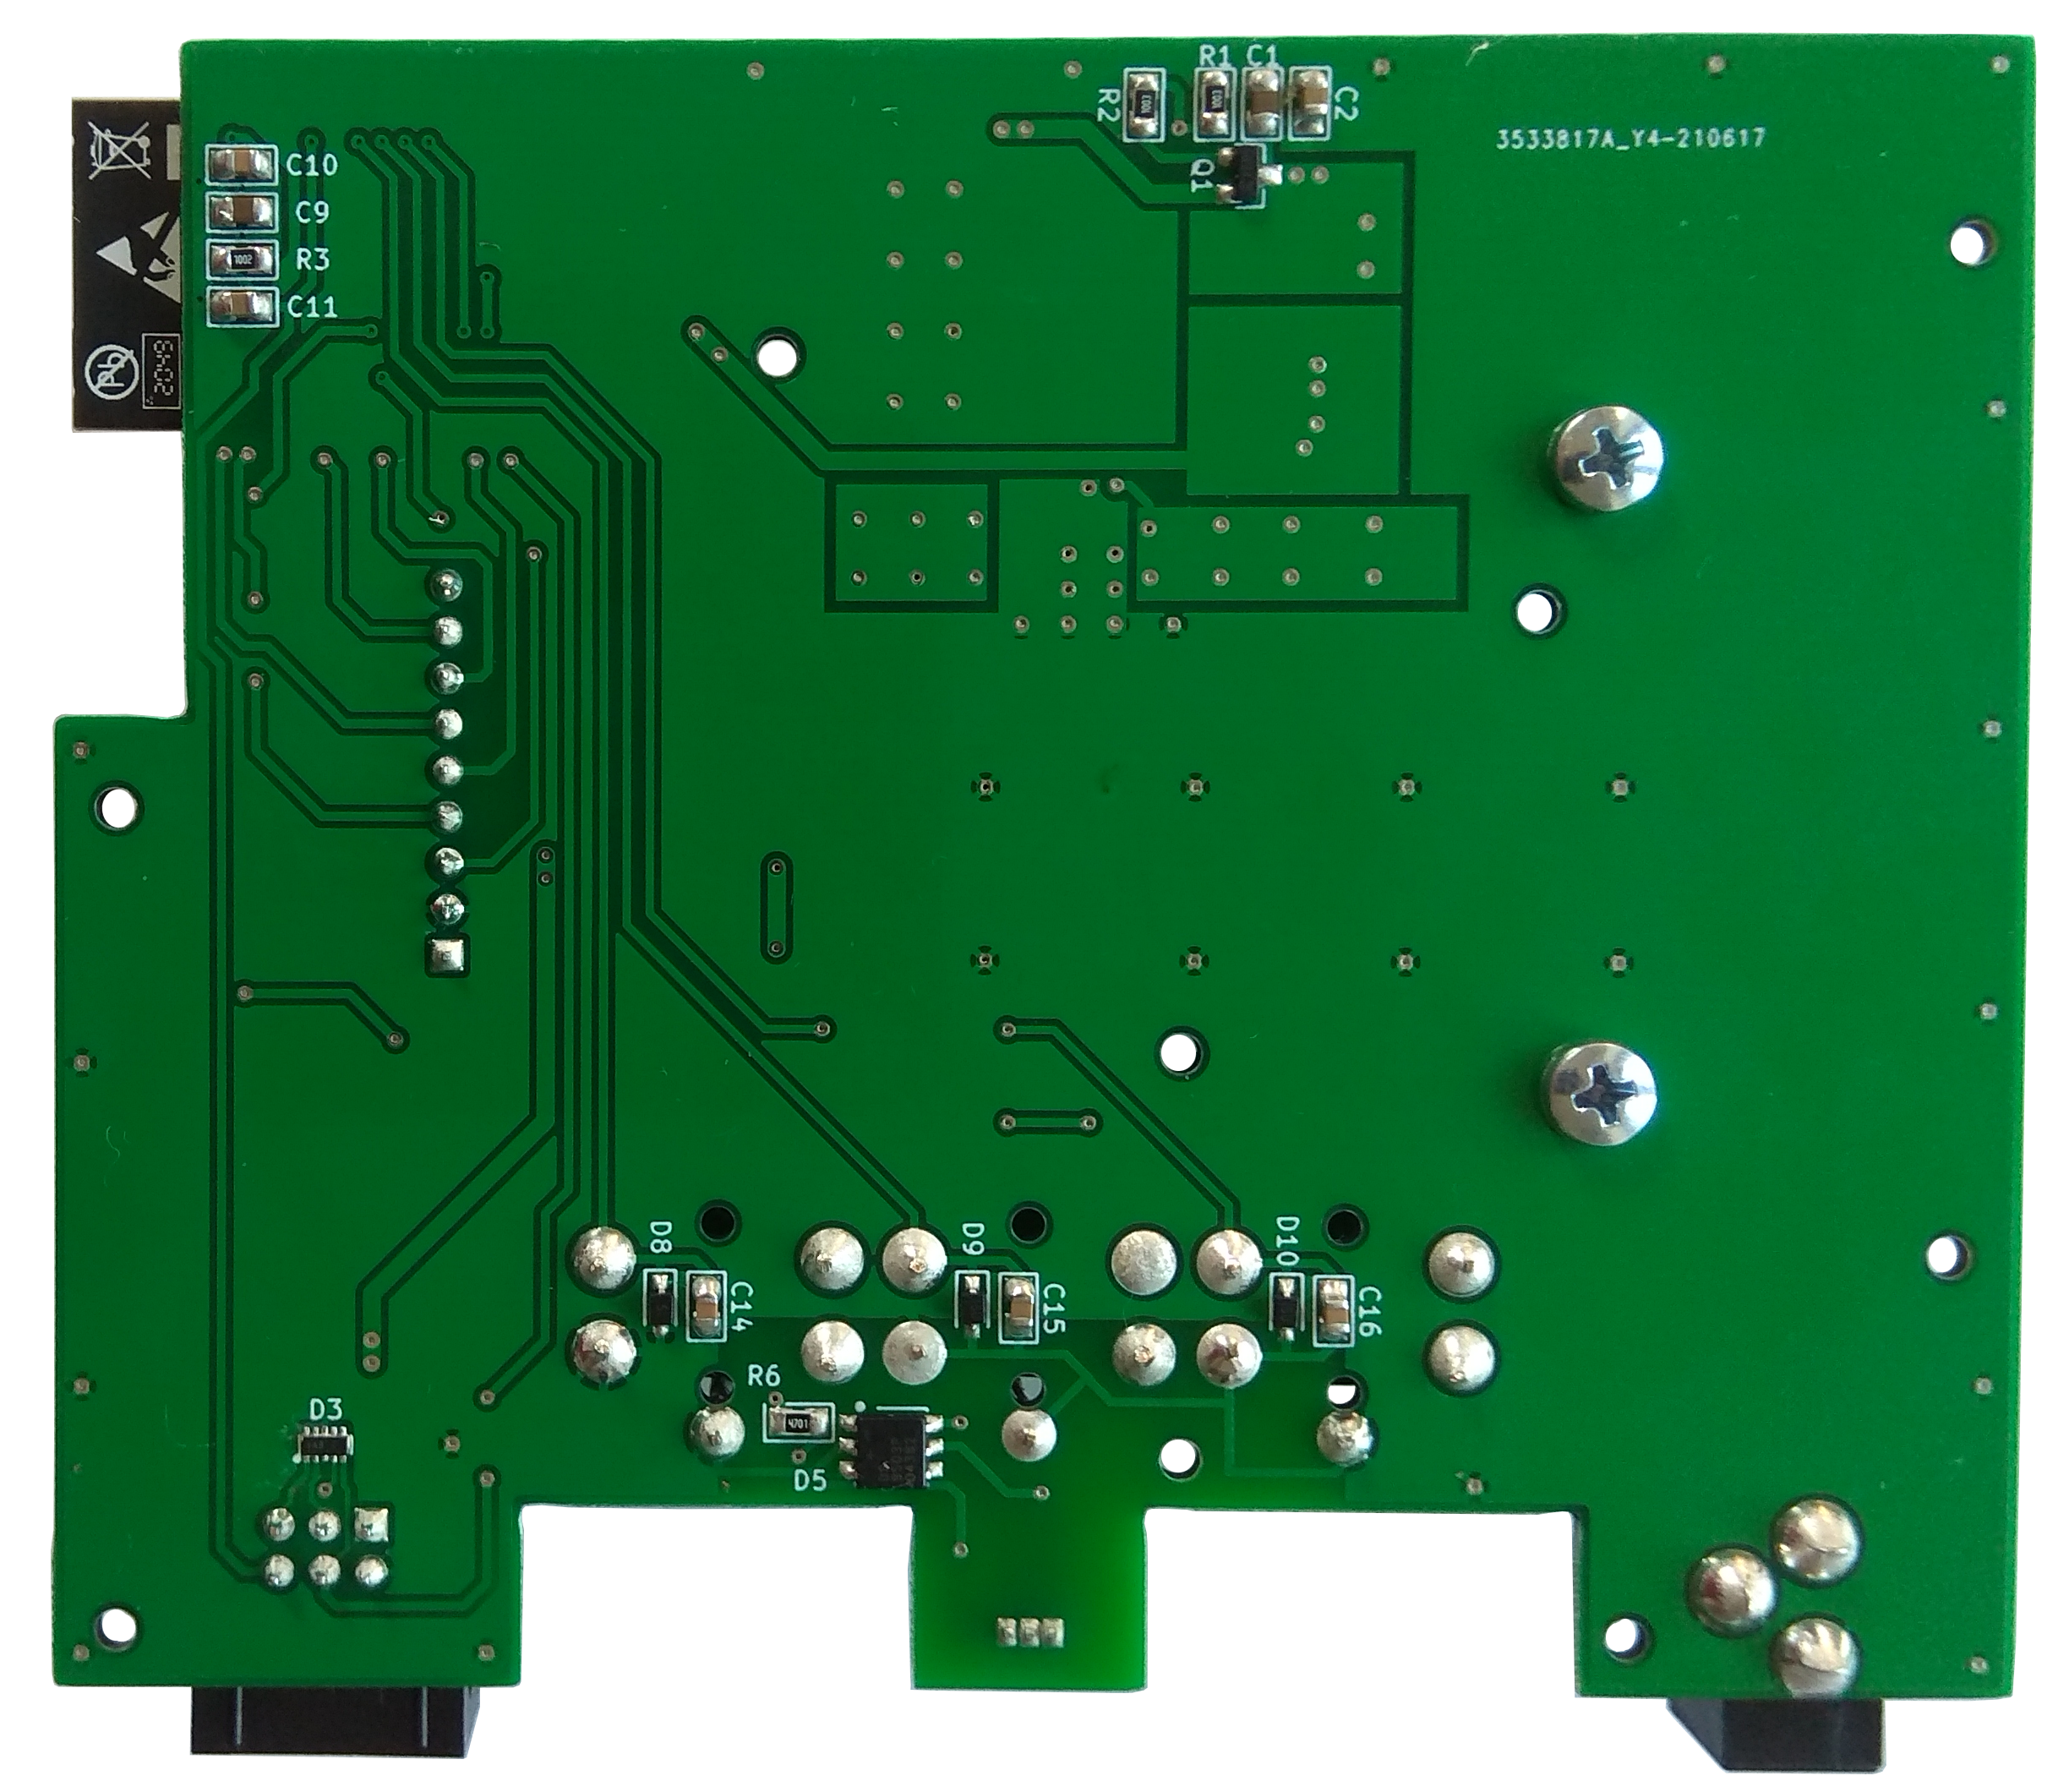
\includegraphics[width=\textwidth]{images/nastenny-snimac-prostorove-teploty-wifi/dps-nastenny-snimac-prostorove-teploty-wifi-spodni-cast.png}
    \caption{Spodní strana.}
    \label{fig:dps-nastenny-snimac-prostorove-teploty-wifi-spodni-cast}
\end{subfigure}
\caption{DPS nástěnného snímače prostorové teploty (verze WiFi).}
\label{fig:dps-nastenny-snimac-prostorove-teploty-wifi}
\end{figure}


\begin{figure}[H]
    \centering
    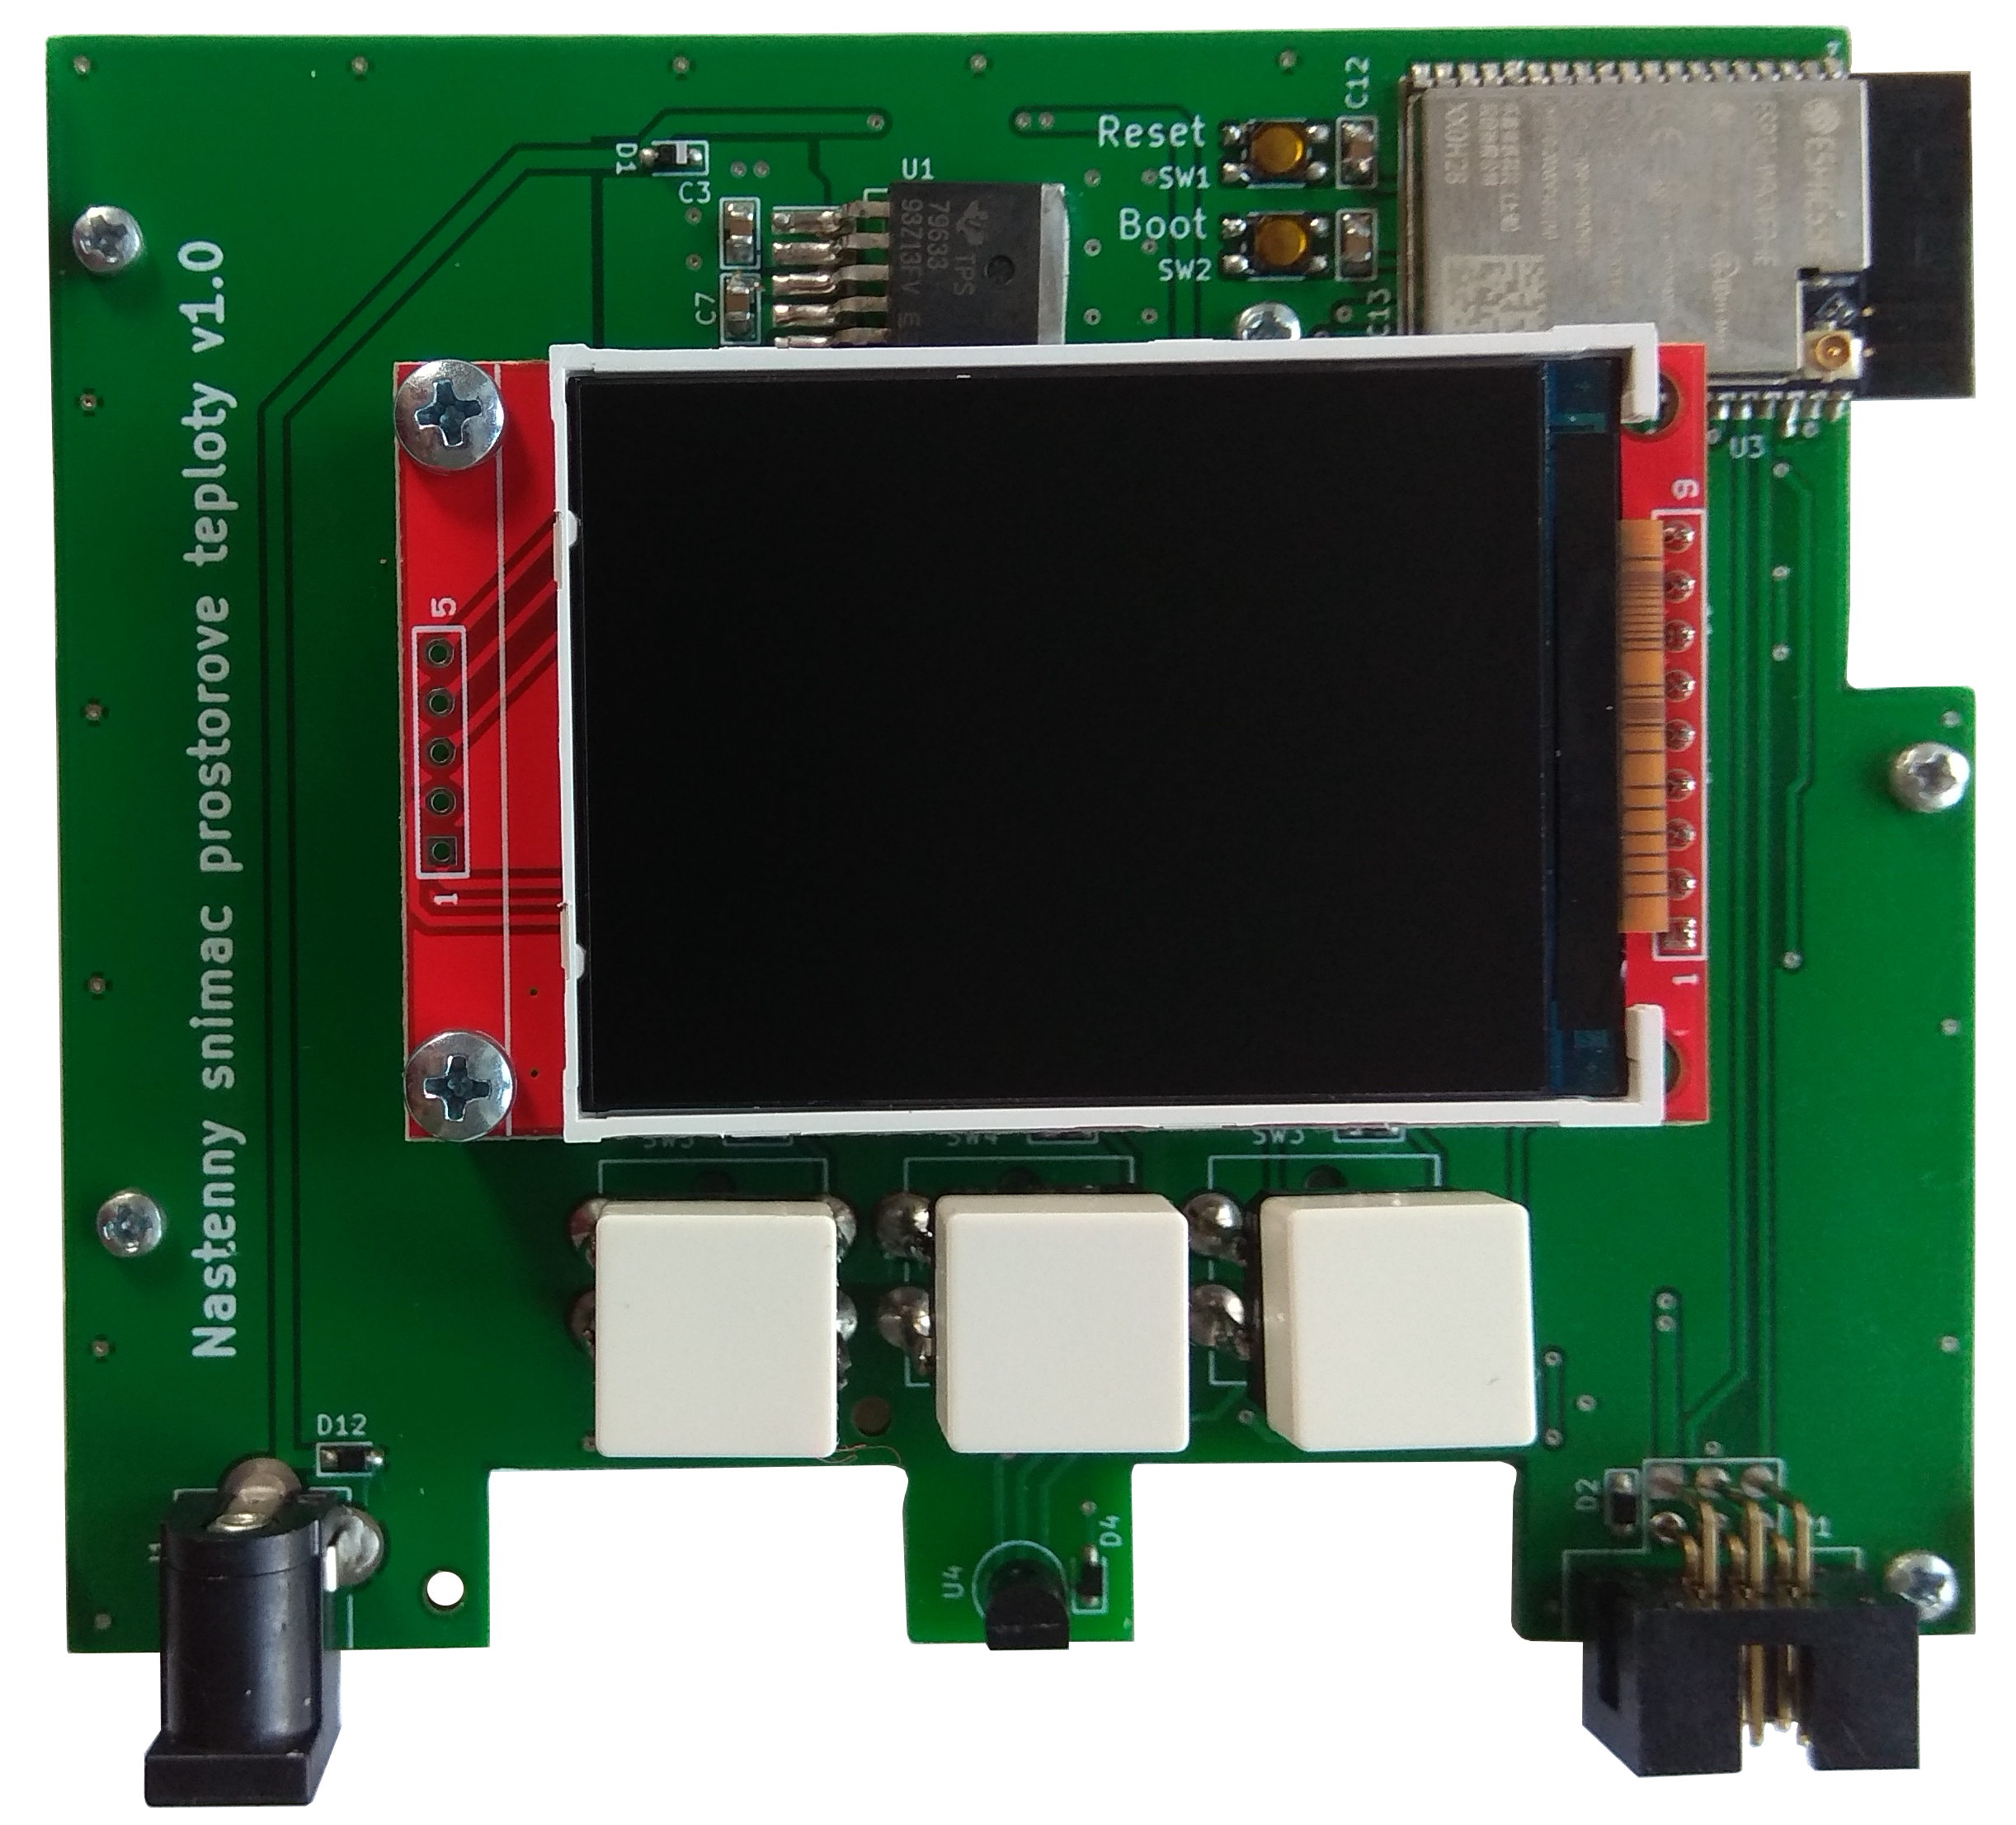
\includegraphics[width=0.85\textwidth]{images/nastenny-snimac-prostorove-teploty-wifi/dps-nastenny-snimac-prostorove-teploty-wifi-vrchni-cast-displej.png}
    \caption{DPS nástěnného snímače prostorové teploty (verze WiFi) s~displejem, vrchní strana.}
    \label{fig:dps-nastenny-snimac-prostorove-teploty-wifi-vrchni-cast-displej}
\end{figure}
\begin{figure}[H]
    \centering
    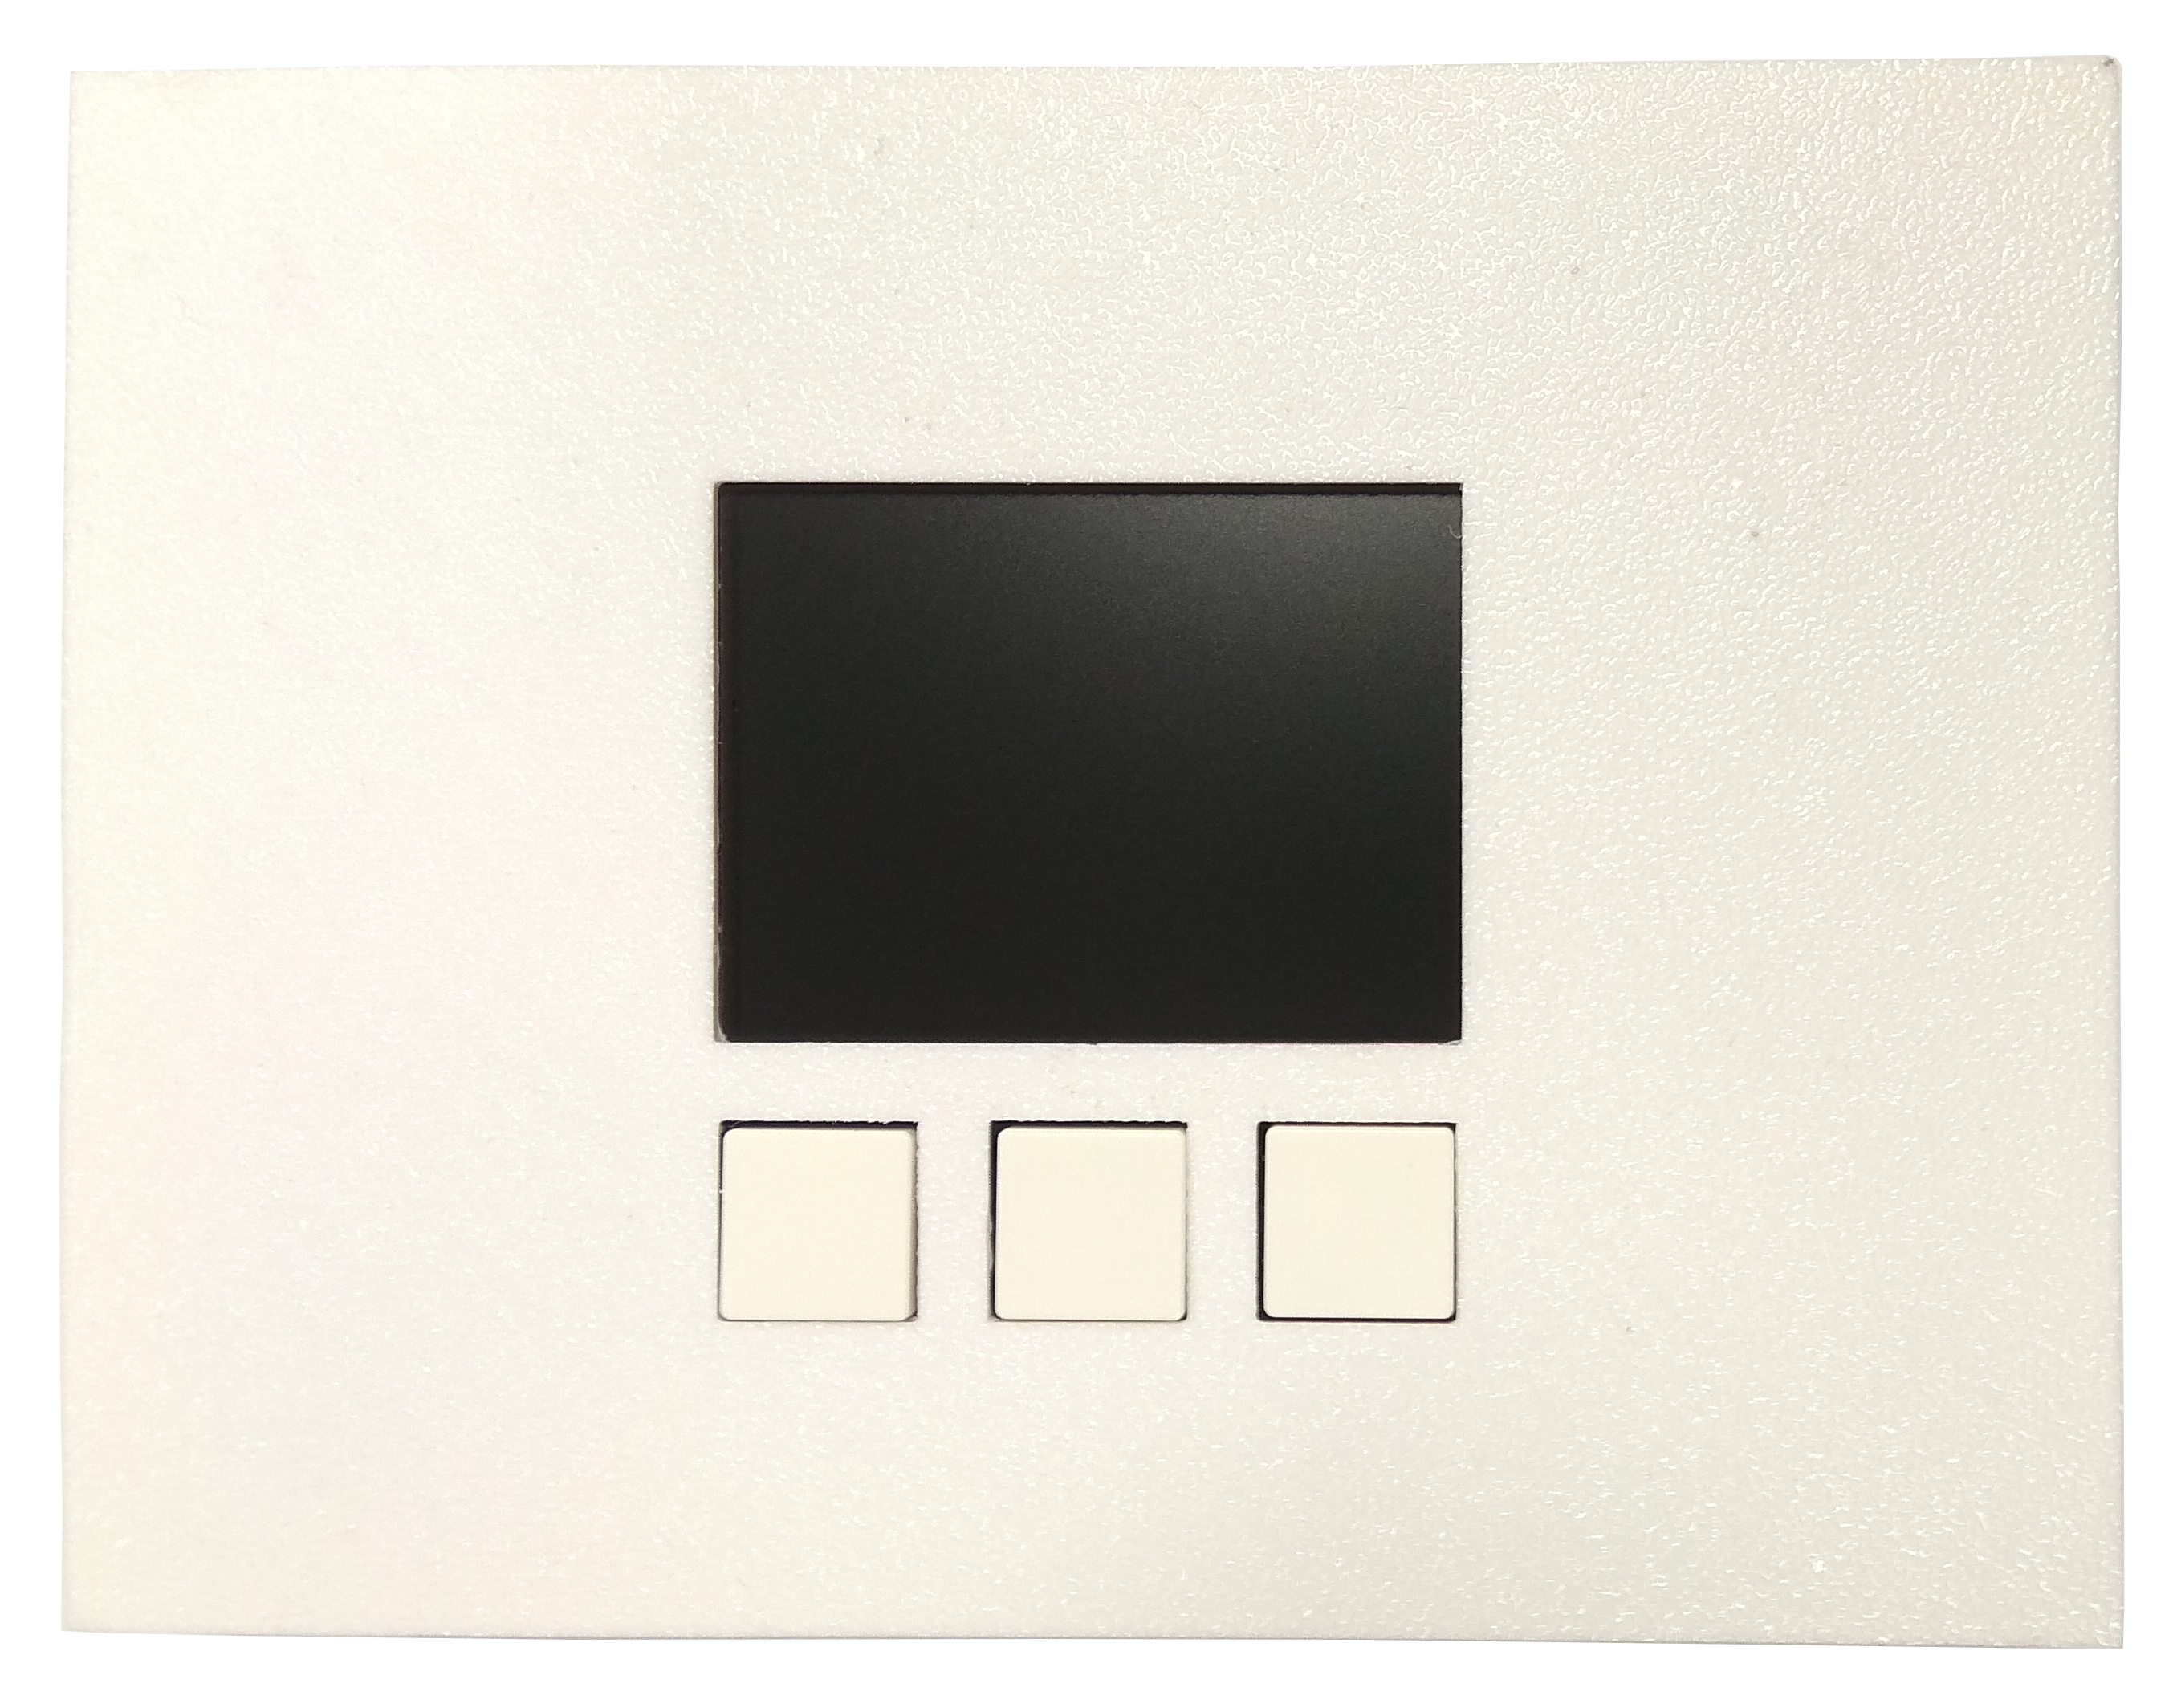
\includegraphics[width=\textwidth]{images/krabicka-nastenny-snimac-prostorove-teploty/krabicka-nastenny-snimac-prostorove-teploty-predni-strana.png}
    \caption{Přední část krabičky.}
    \label{fig:krabicka-nastenny-snimac-prostorove-teploty-predni-strana}
\end{figure}

\begin{figure}[H]
    \centering
    \includegraphics[width=\textwidth]{images/krabicka-nastenny-snimac-prostorove-teploty/krabicka-nastenny-snimac-prostorove-teploty-predni-strana-zezadu.png}
    \caption{Zadní strana přední části krabičky.}
    \label{fig:krabicka-nastenny-snimac-prostorove-teploty-predni-strana-zezadu}
\end{figure}

\begin{figure}[H]
    \centering
    \includegraphics[width=\textwidth]{images/krabicka-nastenny-snimac-prostorove-teploty/krabicka-nastenny-snimac-prostorove-teploty-spodni-cast.png}
    \caption{Spodní část krabičky.}
    \label{fig:krabicka-nastenny-snimac-prostorove-teploty-spodni-cast}
\end{figure}

\begin{figure}[H]
    \centering
    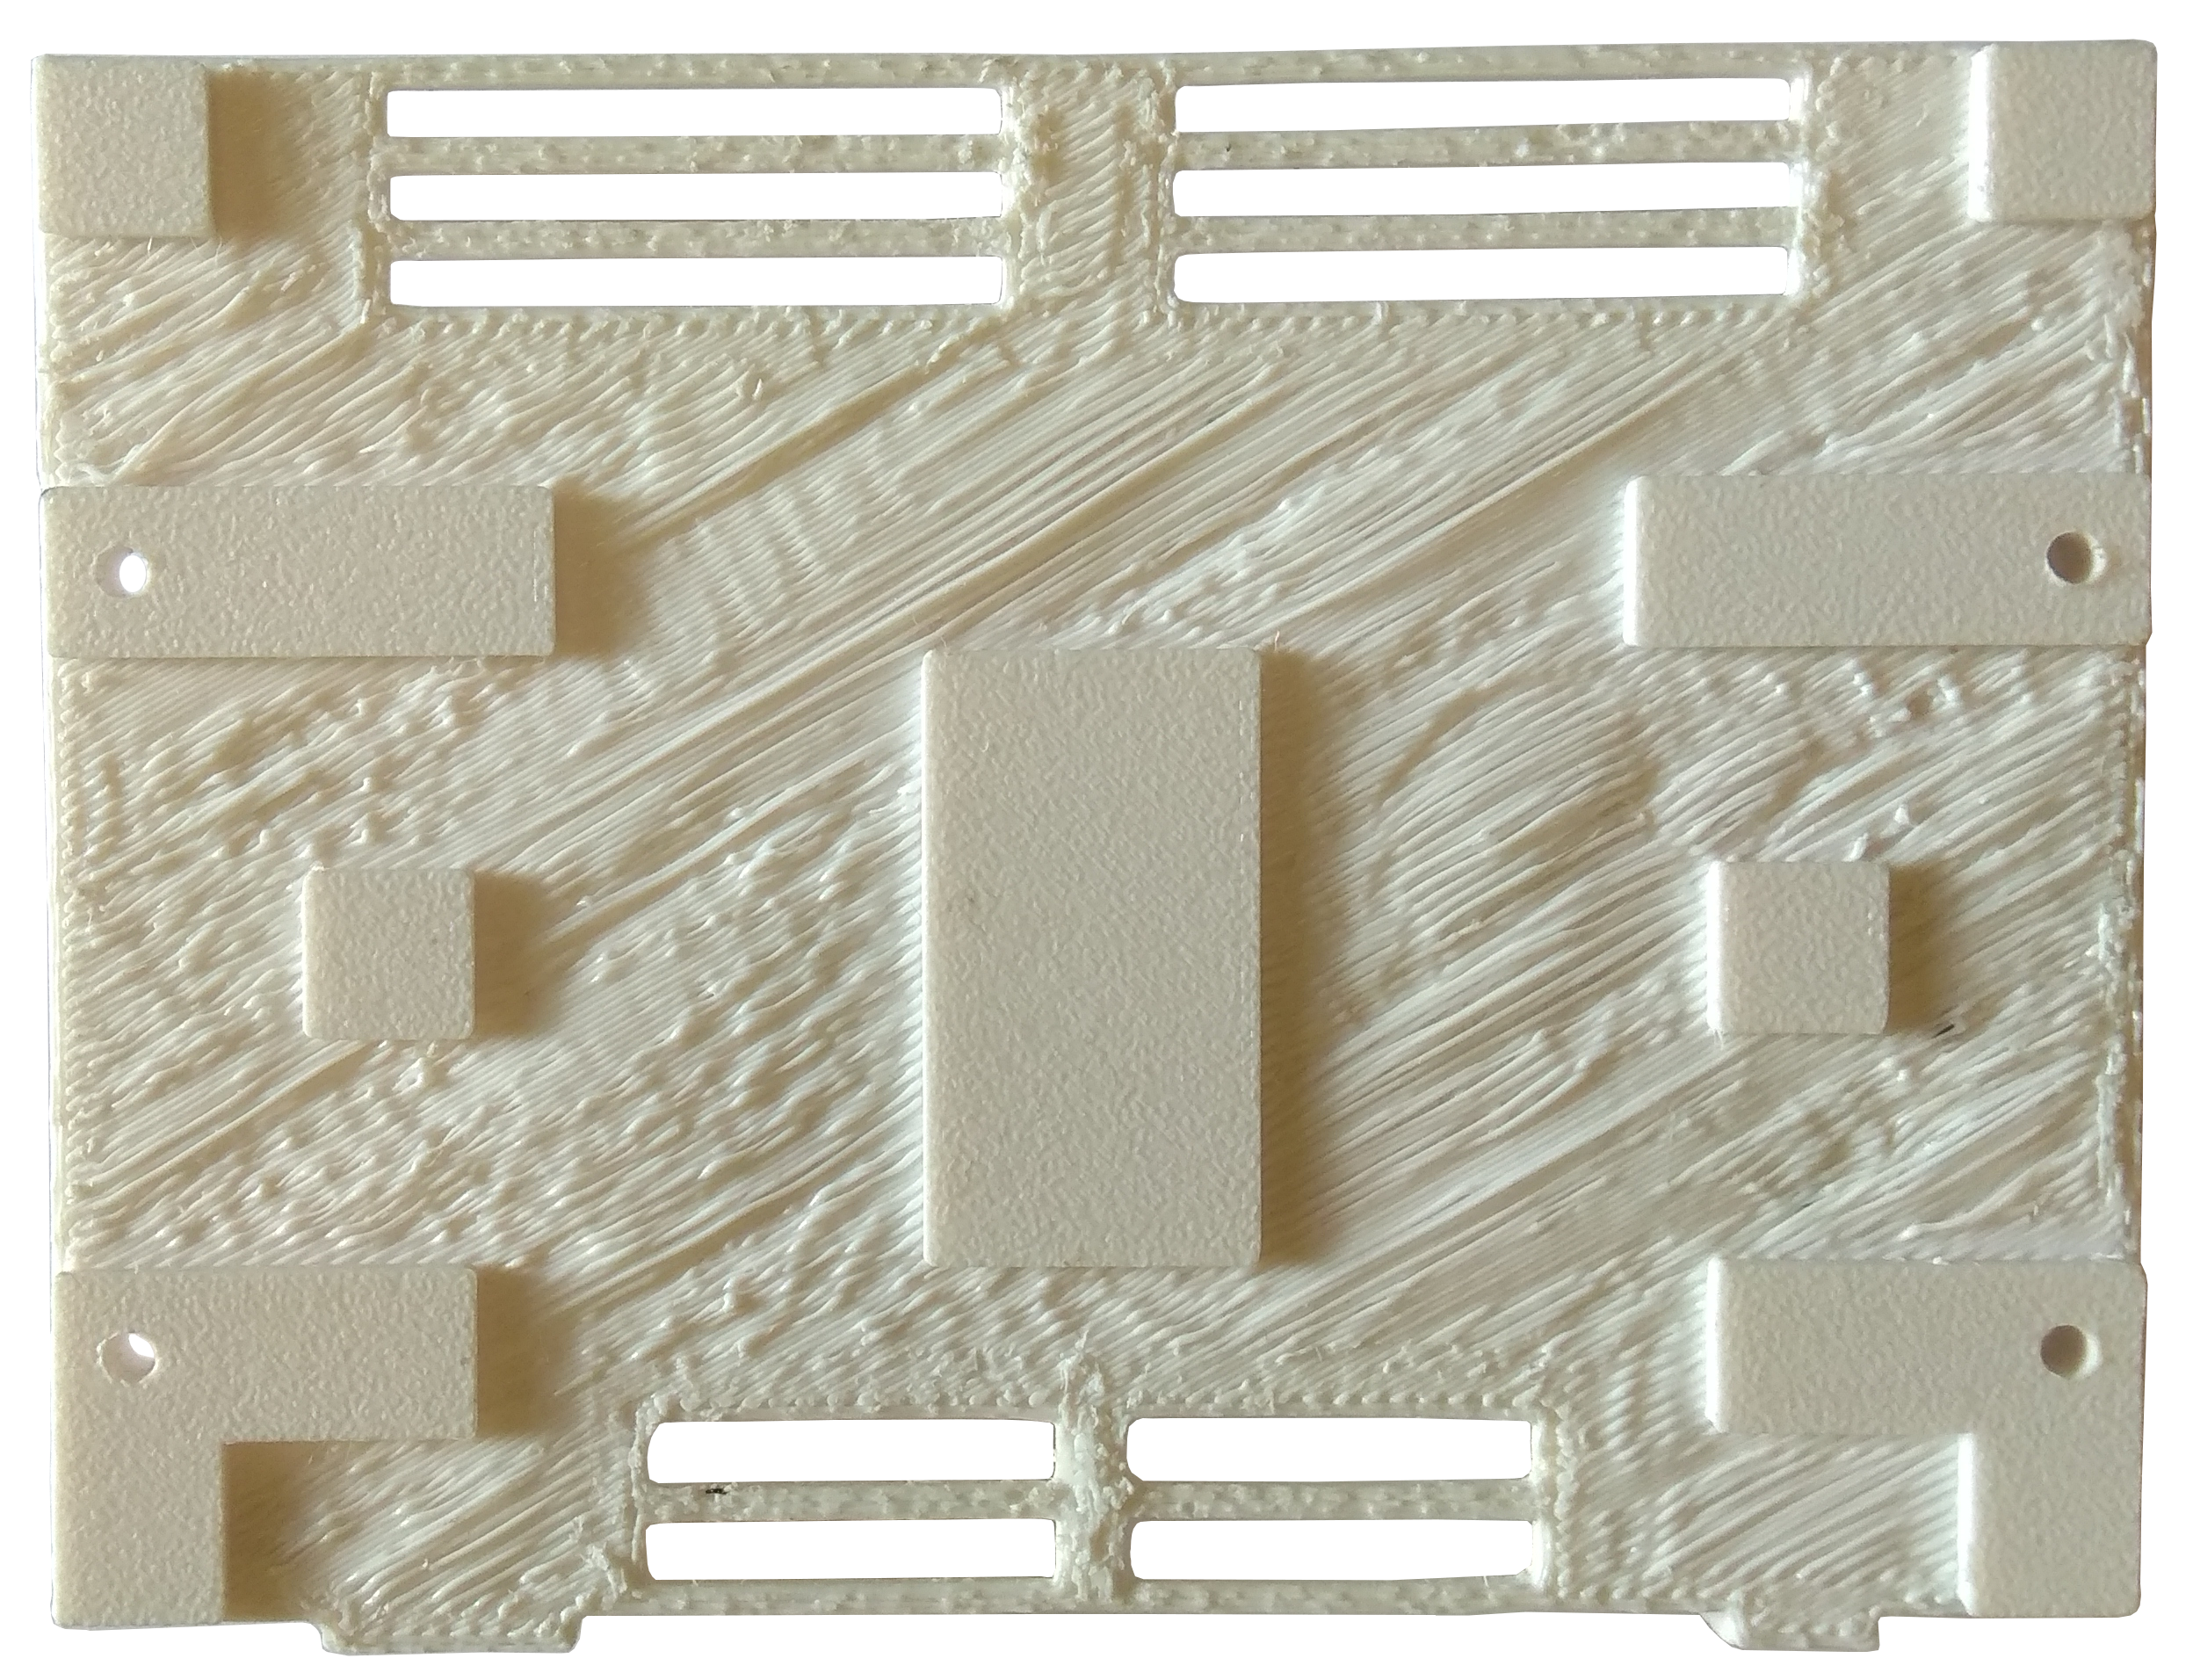
\includegraphics[width=\textwidth]{images/krabicka-nastenny-snimac-prostorove-teploty/krabicka-nastenny-snimac-prostorove-teploty-spodni-cast-zezadu.png}
    \caption{Zadní strana spodní části krabičky.}
    \label{fig:krabicka-nastenny-snimac-prostorove-teploty-spodni-cast-zezadu}
\end{figure}

\begin{figure}[H]
    \centering
    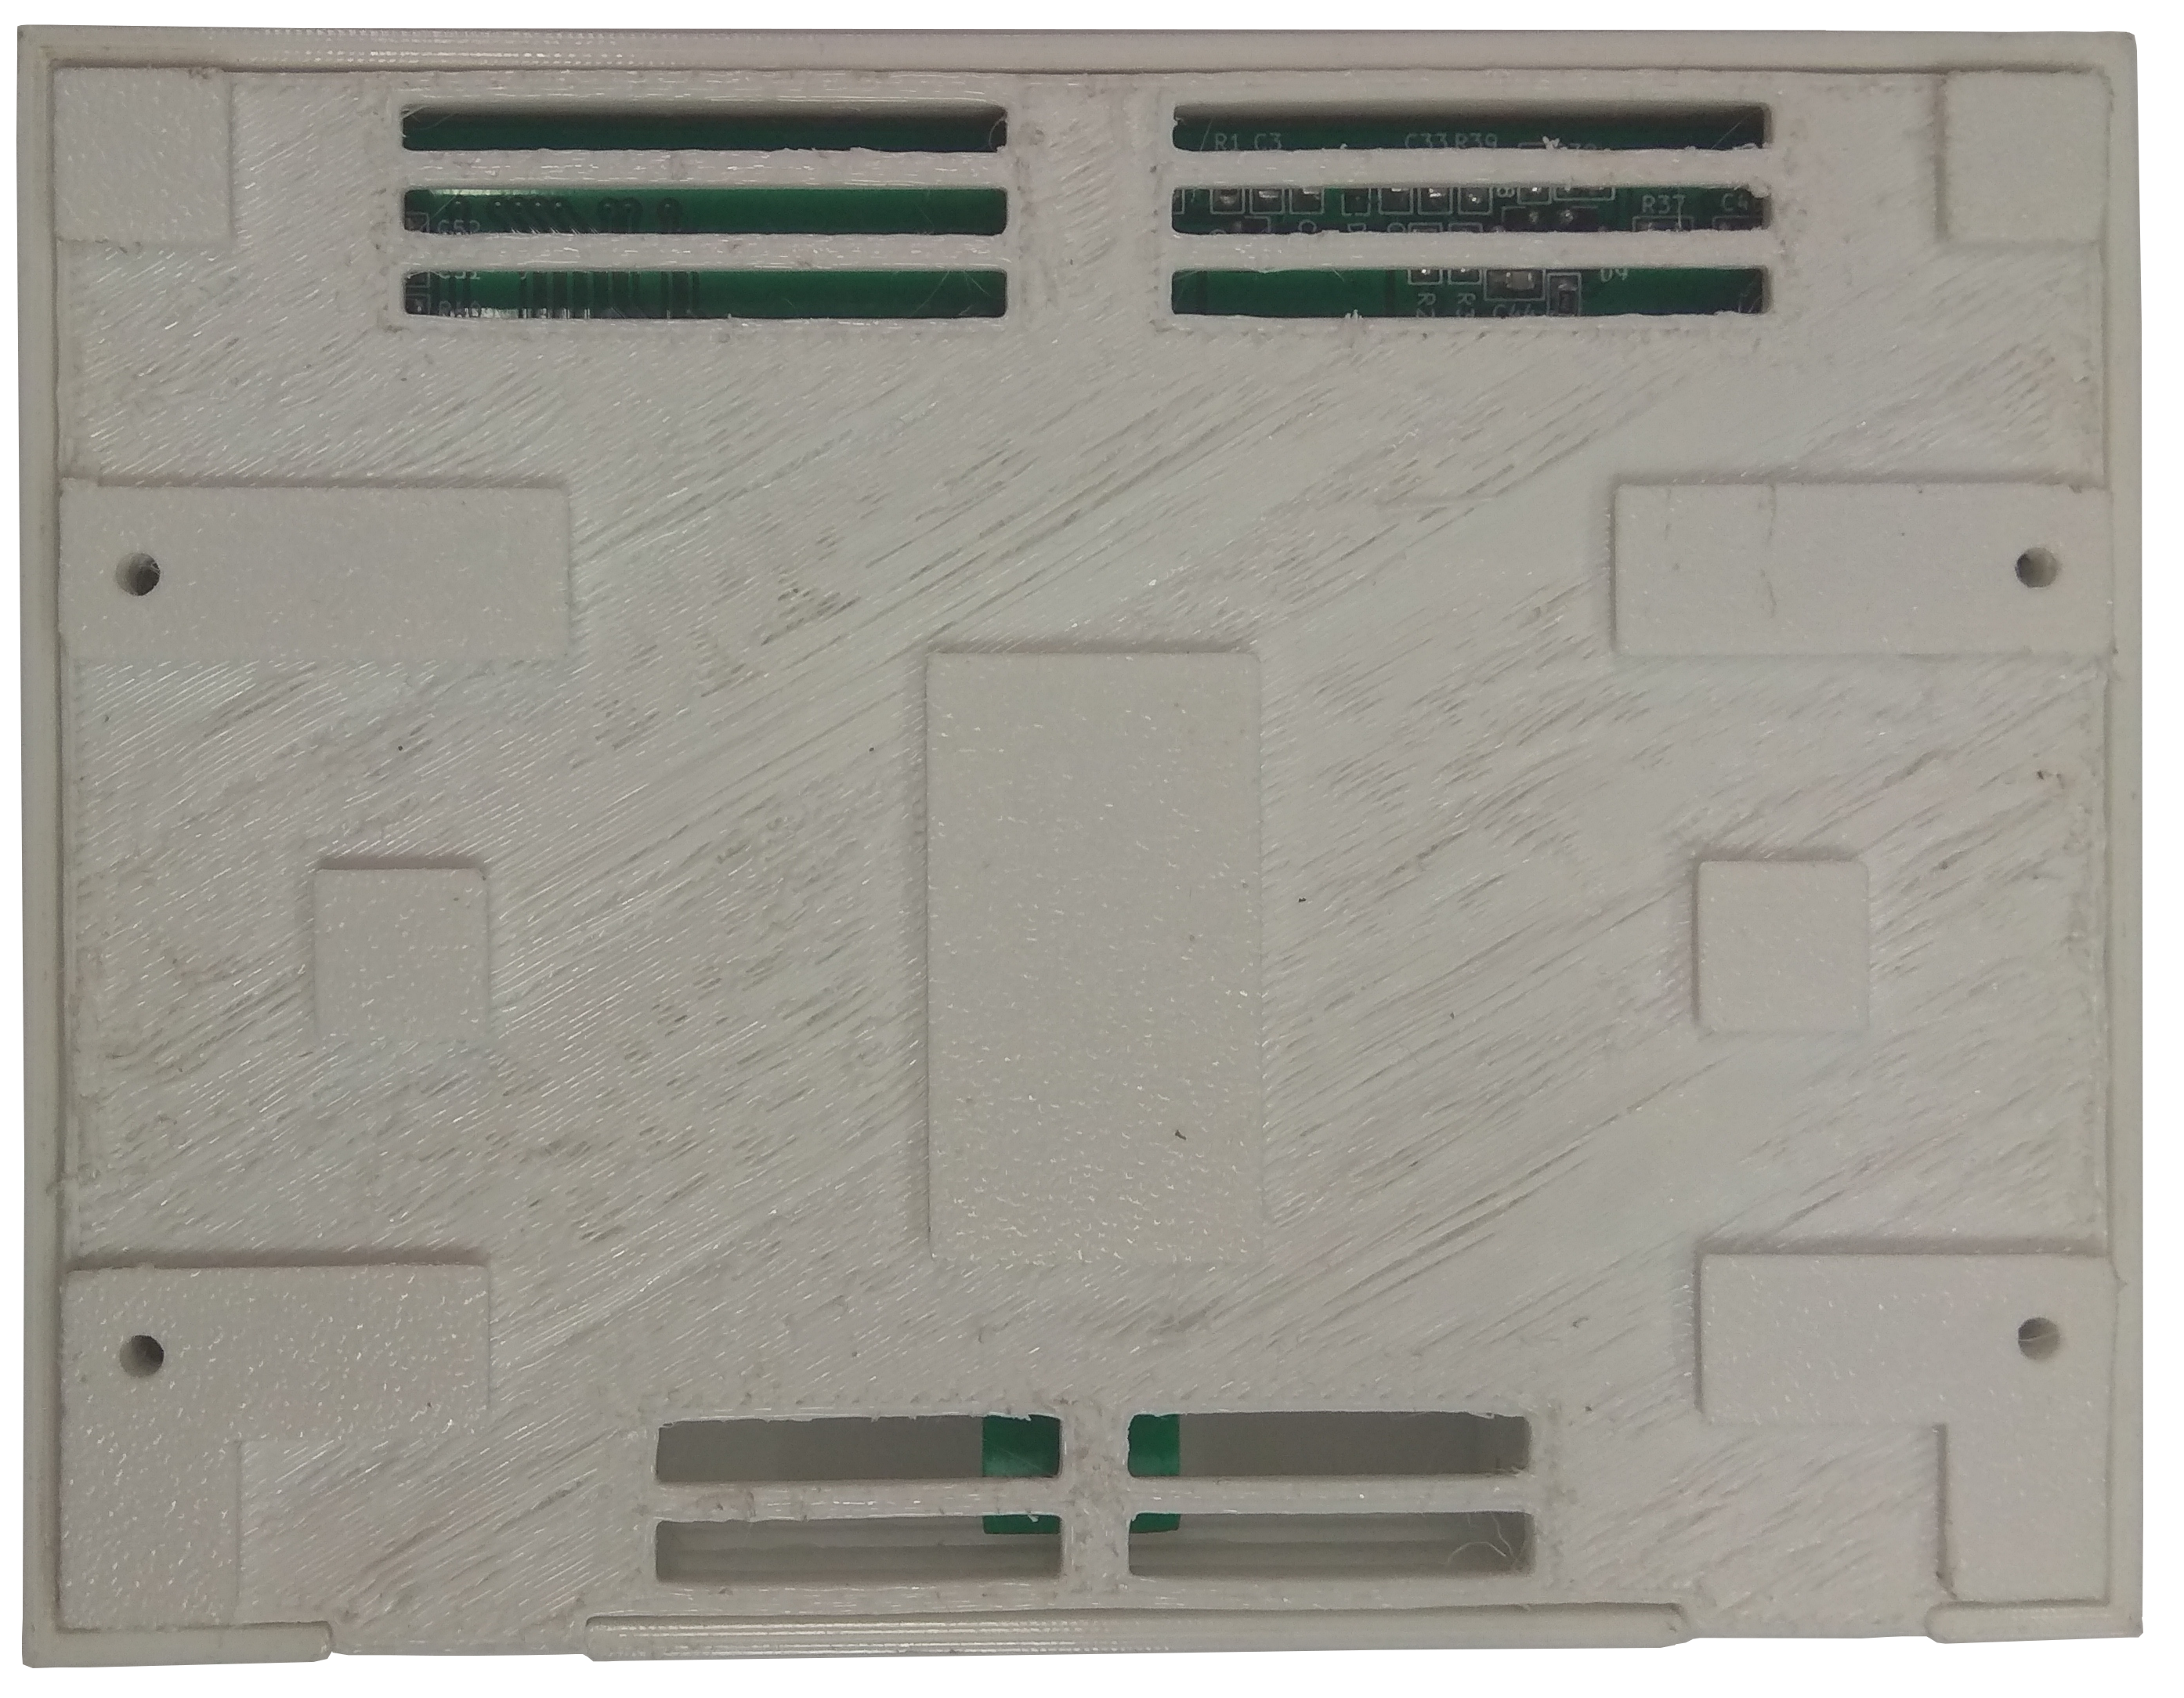
\includegraphics[width=\textwidth]{images/krabicka-nastenny-snimac-prostorove-teploty/krabicka-nastenny-snimac-prostorove-teploty-spodni-cast-zezadu-dps.png}
    \caption{Zadní strana spodní části krabičky s vloženou DPS.}
    \label{fig:krabicka-nastenny-snimac-prostorove-teploty-spodni-cast-zezadu-dps}
\end{figure}

\begin{figure}[H]
    \centering
    \includegraphics[width=\textwidth]{images/krabicka-nastenny-snimac-prostorove-teploty/krabicka-nastenny-snimac-prostorove-teploty-ethernet-celni-strana.png}
    \caption{Čelní strana krabičky, verze s Ethernetem.}
    \label{fig:krabicka-nastenny-snimac-prostorove-teploty-ethernet-spodni-cast-zezadu}
\end{figure}

\begin{figure}[H]
    \centering
    \includegraphics[width=\textwidth]{images/krabicka-nastenny-snimac-prostorove-teploty/krabicka-nastenny-snimac-prostorove-teploty-bocni-strana.png}
    \caption{Boční strana krabičky.}
    \label{fig:krabicka-nastenny-snimac-prostorove-teploty-prava-strana}
\end{figure}

\begin{figure}[H]
    \centering
    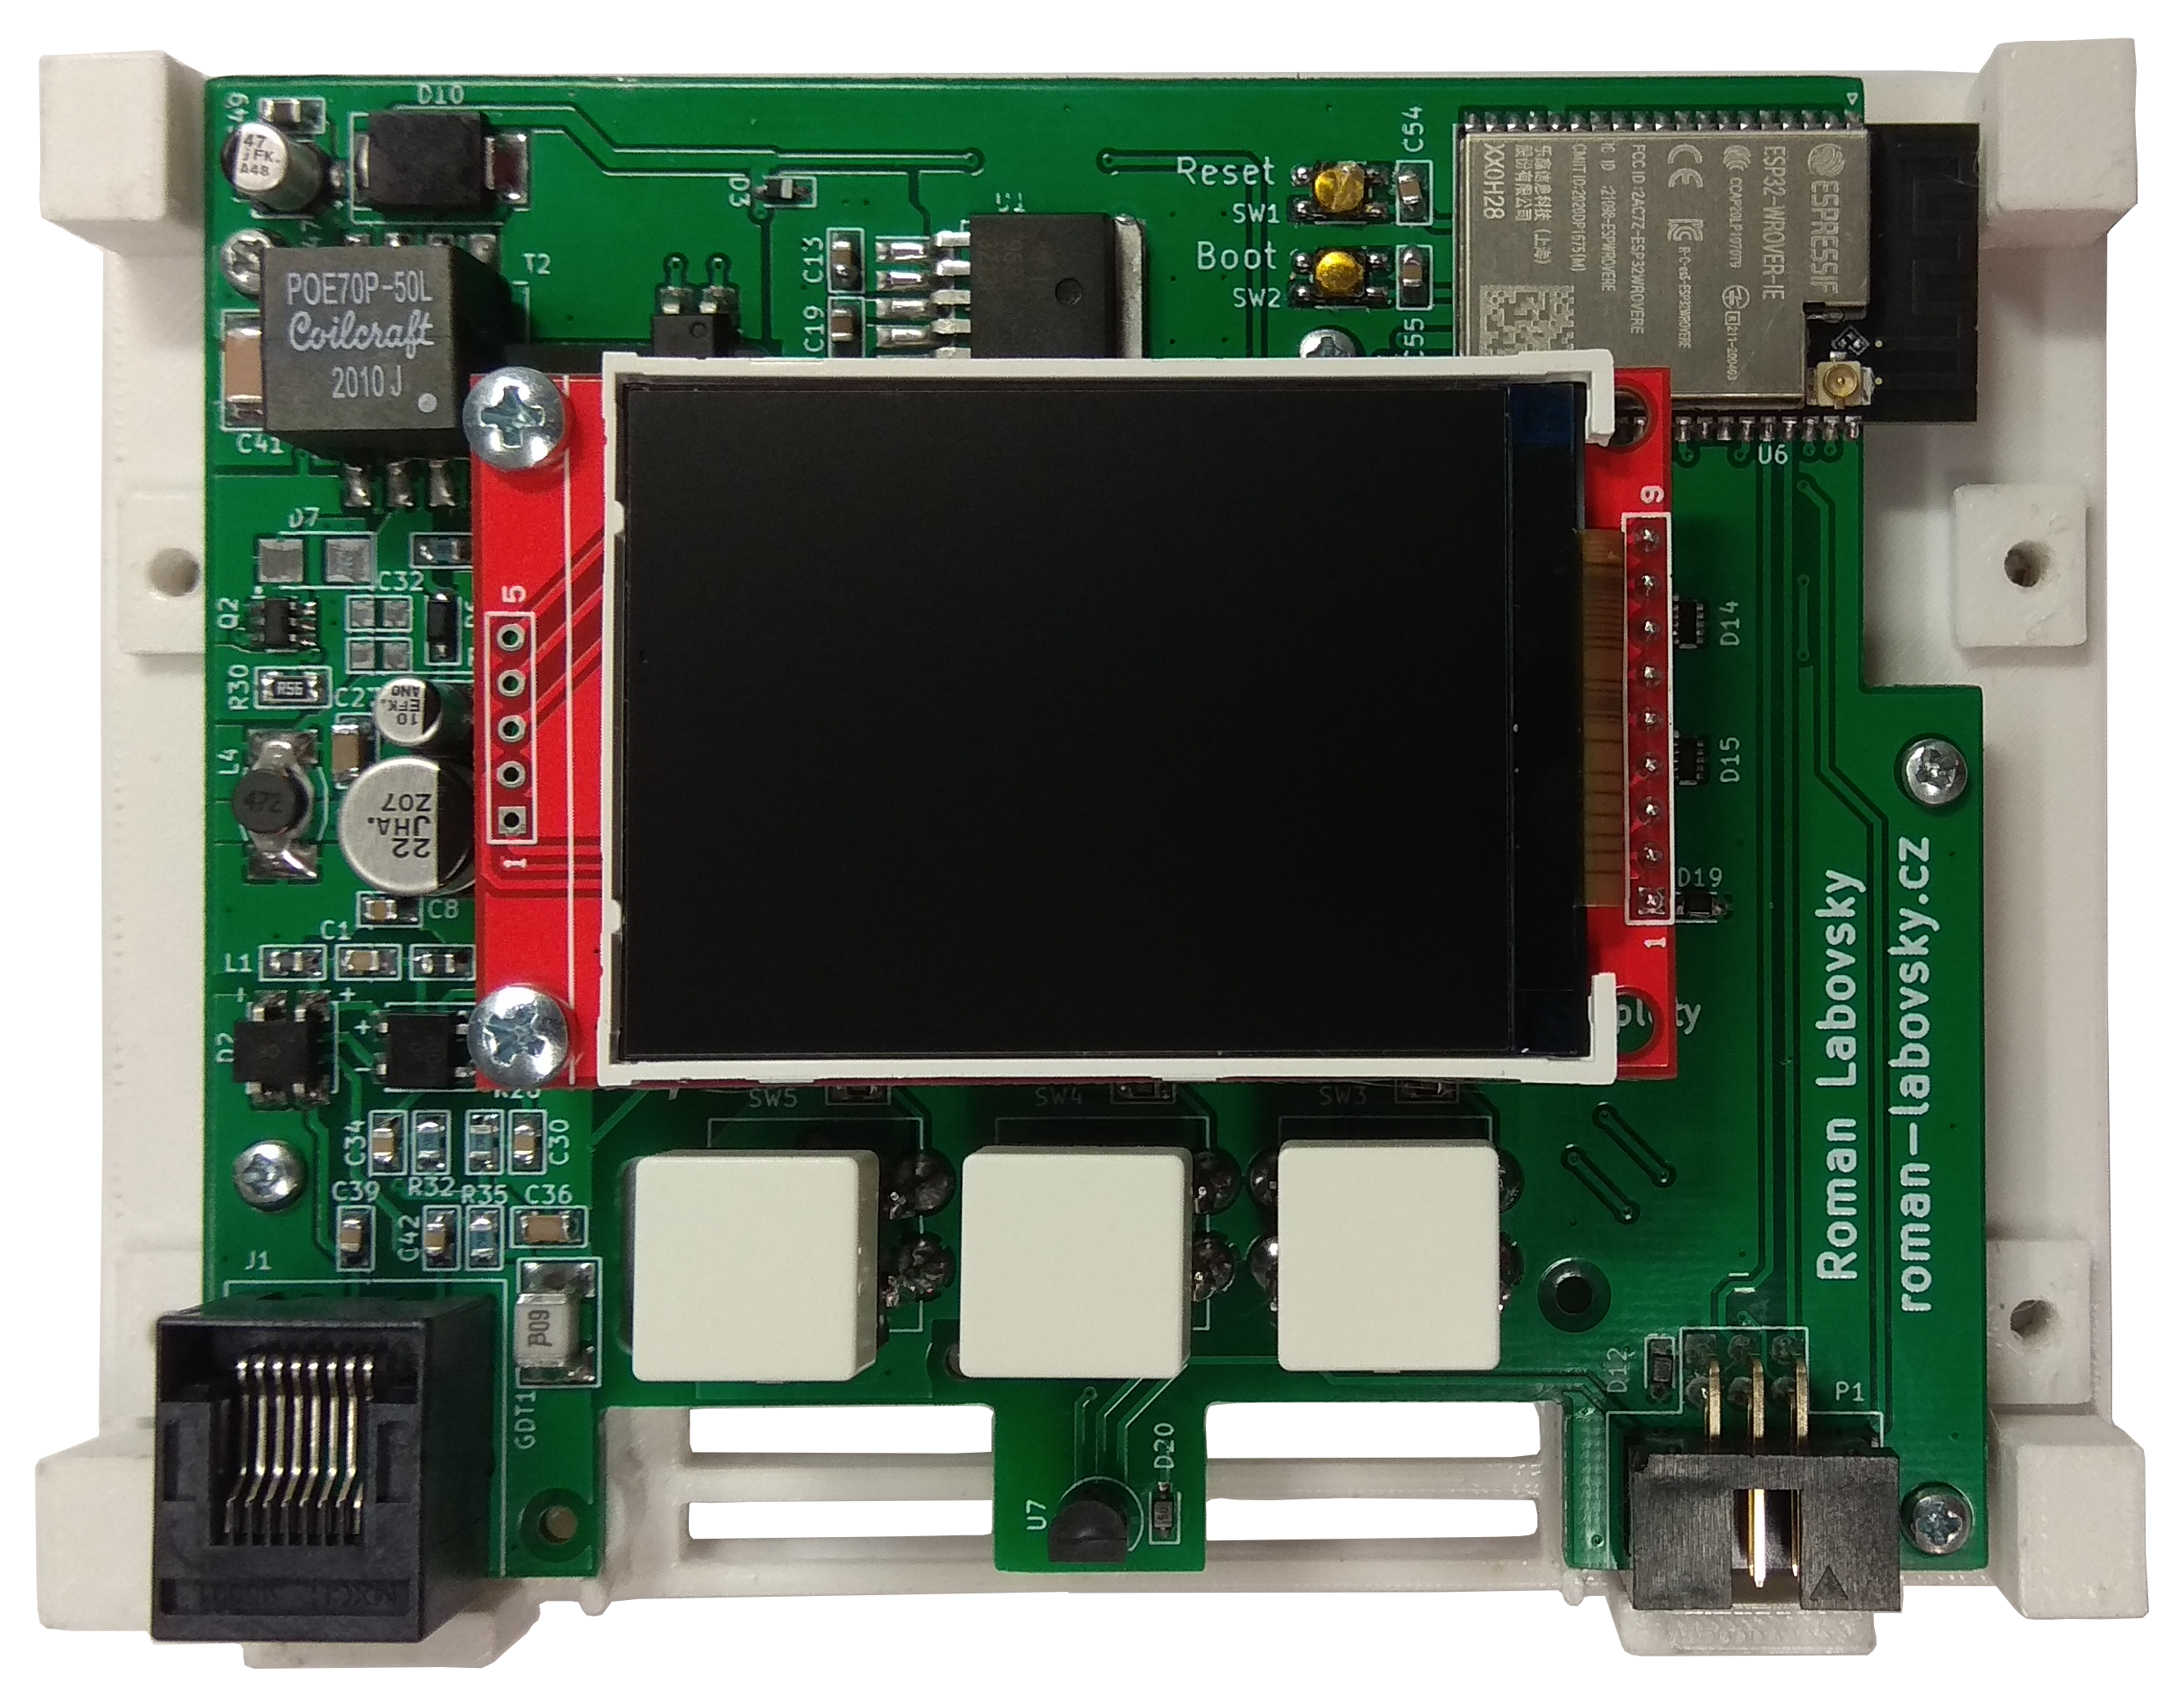
\includegraphics[width=\textwidth]{images/krabicka-nastenny-snimac-prostorove-teploty/krabicka-nastenny-snimac-prostorove-teploty-ethernet-spodni-cast-dps.png}
    \caption{Spodní část krabičky s osazenou DPS.}
    \label{fig:krabicka-nastenny-snimac-prostorove-teploty-ethernet-spodni-cast-dps}
\end{figure}

\begin{figure}[H]
    \centering
    \includegraphics[width=\textwidth]{images/krabicka-nastenny-snimac-prostorove-teploty/krabicka-nastenny-snimac-prostorove-teploty-ethernet-celni-strana-dps.png}
    \caption{Pohled na čelní stranu s osazenou DPS.}
    \label{fig:krabicka-nastenny-snimac-prostorove-teploty-ethernet-celni-strana-dps}
\end{figure}

\begin{figure}[H]
    \centering
    \includegraphics[width=\textwidth]{images/krabicka-nastenny-snimac-prostorove-teploty/krabicka-nastenny-snimac-prostorove-teploty-bocni-strana-dps.png}
    \caption{Boční strana s osazenou DPS.}
    \label{fig:krabicka-nastenny-snimac-prostorove-teploty-bocni-strana-dps}
\end{figure}


\section{Softwarová část}

\subsection{Záložka nastavení}
V části „módy řízení“ se nachází výběr módů a to zimní, letní nebo výběr podle venkovní teploty. Výběr módu má vliv na výběr mezních teplot pro spínání plynového kondenzačního kotle. Dané teplotní meze se dají nastavit v~části „spínání plynového kotle“ (teplotní meze pro léto a zimu). Tyto nastavené meze se berou pro kontrolu s teplotou v horní části zásobníku otopné vody. Pokud teplota v~horní části zásobníku je menší než teplota definovaná v části „min. zapnutí“ dojde k zapnutí kotle pro nahřátí otopné vody, kotel se vypíná při teplota definované v části „max. vypnutí“. Při porovnávání teplot se též bere v potaz nastavená hystereze v části „ostatní nastavení“. Při výběru módu podle venkovní teploty dochází k automatickému výběru letního nebo zimního módu. Teplotní mez pro výběr letního módu (v rámci módu podle venkovní teploty) je definovaná v části „min. venkovní teplota pro letní mód“. 

V části nastavení „krby – spínání čerpadel“ se definují minimální hranice teploty, kdy dojde k sepnutí oběhových čerpadel pro krbové výměníky, tedy při jaké teplotě se má brát v potaz, zda někdo v krbu zatopit a mají se spustit čerpadla pro nahřívání zásobníku otopné vody. Toto nastavení je poměrně důležité a kontrola těchto teplot je zcela nezávislá na dalších nastaveních (automatizaci) v systému, je potřeba vždy při zatopení spustit čerpadla, jinak dojde k přehřátí vody ve výměníku krbu. V případě přehřátí se aktivuje ochrana přímo u krbů a dojde k ke zvukové signalizaci přehřátí, pokud teplota neklesne za určitou dobu, dojde k aktivování ochranných ventilů a vypuštění přehřáté vody.

V části „LED indikace – mezní parametry zásobníku teplé vody se definují mezní teploty pro horní, střední a spodní část zásobníku otopné vody. Tato signalizace se zejména týká pro krby, aby uživatel věděl, zda může topit a jak je moc zásobník nahřátý. U modré LED se definuje mezní minimální teplota, kterou by zásobníku ve horní části měl mít (povolení pro topení). U oranžové LED se definuje mezní maximální teplota, kdy ve střední části zásobníku dochází k dostatečnému nahřátí otopné vody (oznámení, že za chvilku by se mělo přestat topit). U červené LED se definuje mezní maximální teplota, kdy ve spodní části zásobníku je plně ohřátá(okamžitě přestat topit.). Aktivace červené LED předchází v dostatečném předstihu před aktivováním ochrany u~krbů pro přehřátí otopné vody, popsáno v předchozím odstavci.

Pro přehlednost jsou jednotlivé teploty zobrazeny v části „jednotlivé teploty“, jsou zde všechny teploty snímané v zásobníku otopné vody, teploty na kouřovodech v přízemí a patře, v neposlední řadě jez zde i venkovní teplota. V části „porovnání teploty“ jsou zmíněné teploty zobrazeny v jednom grafu.

Výše popsané části jsou zobrazená na obrázku \ref{fig:ha-nastaveni}.


\begin{figure}[H]
    \centering
    \includegraphics[width=\textwidth]{images/software-ha/ha-nastaveni.png}
    \caption{Záložka nastavení v HA.}
    \label{fig:ha-nastaveni}
\end{figure}

\subsection{Záložka zařízení}
V části „koncová zařízení“ se zobrazují jednotlivá ovládána (zapnuto/vypnuto) zařízení otopné soustavy, tedy plynový kondenzační kotel, čerpadla pro krby s výměníkem, čerpadla pro podlahové vytápění a zapnutí signalizačních LED u krbů. Je možné samotnou automatizaci respektive ovládání zmíněných zařízení řídit podle vlastního uvážení, proto slouží přepínač „manuální ovládání zařízení“, zde si pak uživatel může libovolně jednotlivá zařízení ovládat bez ohledu na nastavenou automatizaci.

V části „termostaty chodby – požadavek topení“, zde se zobrazuje zda dochází k vytápění v přízemí či patře na základě nastavení lokálních termostatů na chodbách.

V části „ovládání čerpadel – vodní kámen“ slouží ke spínání čerpadel pro ochranu před zatuhnutím lopatek. Vzhledem k místní dosti tvrdé vodě, došlo při netopení v přízemí, tedy při nevyužívání daných čerpadel k zatuhnutí lopatek v důsledku nánosu vodního kamene. Pro se zde nachází nastavení, kde si uživatel může pro konkrétní den, hodinu a definovanou délku nastavit spínání čerpadel pro odstranění nánosu na lopatách. Ideální volbou je otopnou vodu zbavit minerálů nebo vyměnit za destilovanou vodu, nicméně k některým méně kvalitnějším provedením spojům trubek otopné soustavy, by docházelo k průsaku otopné vody. Proto je otopná vody z řádu s vyšším podílem minerálů jedním z řešení, jak docílit zaslepení průsaku především vápníkem bez nutnosti, alespoň prozatím, spoje opravovat.

Výše popsané části jsou zobrazená na obrázku \ref{fig:ha-zarizeni}.




\begin{figure}[H]
    \centering
    \includegraphics[width=0.90\textwidth]{images/software-ha/ha-zarizeni.png}
    \caption{Záložka zařízení v HA.}
    \label{fig:ha-zarizeni}
\end{figure}

\subsection{Vývoj pro zónovou regulaci}

Na obrázku \ref{fig:teplotni-plan} je zobrazen možný nastavitelný teplotní plán pro celý den. Lze tak nastavit všechny dny v týdnu. Pro každý zvolený teplotní úsek je možné si zvolit požadovanou teplotu.

\begin{figure}[H]
    \centering
    \includegraphics[width=0.90\textwidth]{images/software-ha/teplotni-plan.png}
    \caption{Nastavitelný teplotní plán pro danou hodinu v celém dni.}
    \label{fig:teplotni-plan}
\end{figure}

Na obrázku \ref{fig:termostat-v-mistnosti} je nastavení aktuální teploty pro požadovanou místnost. Každá místnost má svoje vlastní nastavení. Zobrazuje se zde aktuálně naměřená teplota v dané místnosti a požadovaná teplota. Pokud dojde k~přenastavení požadované teploty, dojde k přenesení této teploty do nástěnného snímače prostorové teploty, přenos funguje i opačně.

\begin{figure}[H]
    \centering
    \includegraphics[width=0.90\textwidth]{images/software-ha/termostat-v-mistnosti.png}
    \caption{Zobrazení aktuální teploty z dané místnosti, možnost nastavit požadovanou teplotu.}
    \label{fig:termostat-v-mistnosti}
\end{figure}


